\documentclass[11pt]{report}

\usepackage{mathptmx}
\usepackage{url}
\usepackage{graphicx,pict2e,epic}
\usepackage{verbatim}
\usepackage{wasysym}

\graphicspath{{images/}}

\newcommand*{\p}[1]{\textup{\texttt{#1}}}
\newcommand*{\ls}{\textsc{LearnSAT}}
\newcommand*{\ngg}{\mathop{\neg}}
\newcommand*{\fl}[1]{\parbox{\textwidth}{\raggedleft \p{File: #1}}}

\textwidth=15cm
\textheight=21cm
\topmargin=0pt
\headheight=0pt
\oddsidemargin=5mm
\headsep=0pt
\renewcommand{\baselinestretch}{1.1}
\setlength{\parskip}{0.20\baselineskip plus 1pt minus 1pt}
\parindent=0pt

\setcounter{tocdepth}{1}

\begin{document}

\thispagestyle{empty}

\begin{center}

\textbf{\huge \ls{}\ \ Tutorial}

\bigskip
\bigskip

\textbf{\LARGE Moti Ben-Ari}

\bigskip
\bigskip

\large\url{http: //www.weizmann.ac.il/sci-tea/benari/}

\bigskip

\large Version 2.0


\end{center}

\vspace*{\fill}

\begin{center}
\copyright{} 2012-17 by Moti Ben-Ari.
\end{center}
This work is licensed under the Creative Commons Attribution-ShareAlike 3.0
License. To view a copy of this license, visit
\url{http://creativecommons.org/licenses/by-sa/3.0/}; or, (b) send a letter
to Creative Commons, 543 Howard Street, 5th Floor, San Francisco,
California, 94105, USA.

\newpage

\tableofcontents
\clearpage

%%%%%%%%%%%%%%%%%%%%%%%%%%%%%%%%%%%%%%%%%%%%%%%%%%%%%%%%%%%
%%%%%%%%%%%%%%%%%%%%%%%%%%%%%%%%%%%%%%%%%%%%%%%%%%%%%%%%%%%

\chapter{Overview}

\ls{} is a program for learning about SAT solving. It implements the \emph{Davis-Putnam-Logemann-Loveland (DPLL)} algorithm with \emph{conflict-driven clause learning (CDCL)}, \emph{non-\-chro\-no\-log\-i\-cal backtracking (NCB)} and \emph{lookahead}.

This document is a tutorial on SAT solving with \ls{}. It assumes a basic knowledge of propositional logic such as presented in Chapters~2 and~3 of \cite{mlcs}. This is summarized in Chapter~\ref{ch.intro}. For an introduction to SAT solvers, see \cite[Chapter~6]{mlcs}. The comprehensive reference is the \emph{Handbook of Satisfiability} \cite{SAT}. 

The source programs for \ls{}, the examples and the documentation are contained in an archive \p{learnsat-n.zip}. For instructions on how to run \ls{}, see the \emph{\ls{} User's Guide and Software Documentation} in the archive.

Chapter~\ref{ch.mlm} demonstrates \ls{} in great detail on the example in \cite{mlm}. Chapter~\ref{ch.comb} shows SAT solutions for problems in combinatorics, number theory and graph theory. Chapter~\ref{ch.model} introduces \emph{bounded model checking}, an important application of SAT solving.


%%%%%%%%%%%%%%%%%%%%%%%%%%%%%%%%%%%%%%%%%%%%%%%%%%%%%%%%%%%
%%%%%%%%%%%%%%%%%%%%%%%%%%%%%%%%%%%%%%%%%%%%%%%%%%%%%%%%%%%

\chapter{Propositional logic}\label{ch.intro}

In this chapter we give an overview of propositional logic needed to study SAT solving. Sections~\ref{s.syntax} and~\ref{s.semantics} present the syntax and semantics that should be familiar, although clausal form may be new. Section~\ref{s.theorems} gives some important algorithms and theorems concerning clausal form. Section~\ref{s.dpll} introduces the \emph{DPLL} algorithm upon which most SAT solving algorithms are based.

%%%%%%%%%%%%%%%%%%%%%%%%%%%%%%%%%%%%%%%%%%%%%%%%%%%%%%%%%%%

\section{Syntax}\label{s.syntax}

\begin{itemize}
\item $\mathcal{P}=\{p_1,p_2,\ldots\}$ is a set of elements $p_i$ called \emph{variables}, \emph{atomic propositions} or \emph{atoms}.
\item There is a unary operator \emph{negation}, denoted $\ngg$. $\ngg x$ is the negation of the atom $p$. A negated atom is also denoted $\bar{p}$.
\item A \emph{literal} is an atom $p$ or the negation of an atom $\ngg p$. 
\item An atom is a \emph{positive literal} and the negation of an atom
is a \emph{negative literal}.
\item Let $l$ be a literal. $l^c$, the \emph{complement} of $l$, is $\ngg p$ if
$l=p$ for some atom p and is $p$ if $l=\ngg p$.
\item $l$ and $l^c$ are a \emph{complementary pair of literals}.
\item There are two binary operators: \emph{disjunction}, denoted $\vee$, and \emph{conjunction}, denoted $\wedge$.
\item A \emph{clause} is the disjunction of a set of literals: $l_1 \vee \cdots \vee l_n$, such as $\ngg p_1 \vee \ngg p_2 \vee p_3$. A clause can be written using set notation, for example, $\{\bar{p_1}, \bar{p_2}, p_3\}$.
\item The \emph{empty clause} $\Box$ is the clause that is the empty set.
\item (Syntactic definition) A \emph{unit clause} is a clause that has exactly one literal $\{l\}$.
\item A \emph{formula} in \emph{conjunctive normal form (CNF)} or in \emph{clausal form} is the conjunction of a set of clauses:
\[
(p1 \vee \ngg p_2) \; \wedge \; (\ngg p_1 \vee \ngg p_2 \vee p_3) \;\wedge\; (\ngg p_3)\,.
\]
Nested set notation can be used for formulas in clausal form:
\[
\{\;\{p1, \bar{p_2}\}, \; \{\bar{p_1}, \bar{p_2}, p_3\}, \; \{\bar{p_3}\}\;\}\,.
\]

\item The \emph{empty formula} $\emptyset$ is the formula that is the empty set.

\item Let $C_{1},C_{2}$ be clauses such that $l\in C_{1},l^{c}\in C_{2}$. $C$, the \emph{resolvent} of $C_{1}$ and $C_{2}$, is the clause $(C_{1}-\{l\}) \cup (C_{2}-\{l^{c}\})$. $C_{1}$ and $C_{2}$ are the \emph{parent clauses} of $C$. $C_{1}$ and $C_{2}$ are \emph{clashing clauses} that \emph{clash} on the literals $l,l^c$.


\end{itemize}

%%%%%%%%%%%%%%%%%%%%%%%%%%%%%%%%%%%%%%%%%%%%%%%%%%%%%%%%%%%

\section{Semantics}\label{s.semantics}

The semantics of a formula in propositional logic are specified by interpretations that assign \emph{truth values} to the atoms, and then the assignment is extended to formulas. The extension is defined in terms of clauses, but they are easy to understand if you translate clauses into disjunctions of literals and formulas into conjunctions of clauses.

\begin{itemize}

\item An \emph{interpretation} is a function $\mathcal{I}: \mathcal{P}
\rightarrow \{T,F\}$.

\item The mapping of an interpretation is extended to literals, clauses and formulas as follows:

\begin{itemize}
\item $\mathcal{I}(l)=T$, the literal $l$ is \emph{true} in the
interpretation $\mathcal{I}$, if $l$ is an atom $p$ and $\mathcal{I}(p)=T$, or if $l$ is the negation of an atom $\bar{p}$ and $\mathcal{I}(p)=F$. $\mathcal{I}(l)=F$, $l$ is \emph{false} in $\mathcal{I}$, if $l$ is an atom $p$ and $\mathcal{I}(p)=F$, or if $l$ is the negation of an atom $\bar{p}$ and $\mathcal{I}(p)=T$

\item $\mathcal{I}(C)=T$, the clause $C$ is \emph{true} in the
interpretation $\mathcal{I}$, if for \emph{at least one} $l\in C$,
$\mathcal{I}(l)=T$. $\mathcal{I}(C)=F$, $C$ is \emph{false} in $\mathcal{I}$, if for \emph{all} $l\in C$, $\mathcal{I}(l)=F$.

\item $\mathcal{I}(A)=T$, the formula $A$ is \emph{true} in the
interpretation $\mathcal{I}$, if for \emph{all} $C \in A$,
$\mathcal{I}(C)=T$. $\mathcal{I}(A)=F$, $A$ is \emph{false} in $\mathcal{I}$, if for \emph{at least one} $C\in A$, $\mathcal{I}(C)=F$.

\end{itemize}

\item A formula $A$ is \emph{satisfiable} if there exists an
interpretation $\mathcal{I}$ such that $\mathcal{I}(A)=T$. If there is
no such interpretation, $A$ is \emph{unsatisfiable}.

\item $\mathcal{I}$ is a \emph{partial interpretation} for $A$ if it
maps \emph{some} of the atoms in $A$ into $\{T,F\}$.
A partial interpretation can assign truth values to enough atoms so that the truth value of $A$ can be computed. For example, given the formula:
\[
A=\{\;\{p1, \bar{p_2}\}, \; \{\bar{p_1}, \bar{p_2}, p_3\}, \; \{\bar{p_3}\}\;\}\,,
\]
under the partial interpretation $\{\mathcal{I}(p_2)=F, \mathcal{I}(p_3)=F\}$, $\mathcal{I}(A)=T$, and under the partial interpretation $\{\mathcal{I}(p_3)=T\}$, $\mathcal{I}(A)=F$.

\item Let $A$ be a formula and let $\mathcal{I}$ be a partial
interpretation for $A$. $A'=\mathcal{I}(A)$, the formula obtained by
\emph{evaluating $A$ under $\mathcal{I}$}, is obtained by removing all
clauses $C\in A$ such that for some $l\in C$, $\mathcal{I}(l)=T$, and by
removing from the remaining clauses all literals $l'$ such
$\mathcal{I}(l')=F$. The justifications for this definition and the next one are given in the Section~\ref{s.theorems}.

\item (Semantic definition) A clause $C$ is a \emph{unit clause} under a partial interpretation $\mathcal{I}$ if for some $l\in C$, the atom of $l$ is not in the domain of $\mathcal{I}$ and if for all $l'\in C, l'\neq l$, $\mathcal{I}(l')=F$.

\item A \emph{decision procedure} for satisfiability is an algorithm that returns \emph{satisfiable} or \emph{unsatisfiable} when a formula is the input to the procedure. When a formula is satisfiable, the decision procedure should return a (possibly partial) interpretation that satisfies the formula.

\item A decision procedure is \emph{sound} if the output \emph{satisfiable} is returned only for satisfiable formulas, and it is \emph{complete} if the output \emph{satisfiable} is returned for every satisfiable formula.

\item The \emph{SAT} problem is to construct a sound and (hopefully) complete decision procedure for satisfiability. The procedure is called a \emph{SAT solver}. Truth tables can be used as a sound and complete SAT solver, but are always inefficient.

\item The SAT problem is $\mathcal{NP}$-complete so it is unlikely that there is an efficient algorithm for satisfiability. Nevertheless, there are algorithms that are efficient on many classes formulas.

\end{itemize}

%%%%%%%%%%%%%%%%%%%%%%%%%%%%%%%%%%%%%%%%%%%%%%%%%%%%%%%%%%%

\section{Theorems}\label{s.theorems}

\textbf{Unit clause rule} Let $A$ be a formula, $C=\{l\}$ a unit clause in $A$, and $\mathcal{I}$ a partial interpretation that does not assign a value to $l$. Construct $\mathcal{I}'$ as the (possibly partial) interpretation obtained by adding an assignment to $l$ to $\mathcal{I}$ such that $\mathcal{I}'(l)=T$. Construct $A'$ by deleting the unit clause $C$ and deleting $l^{c}$ from every clause in which it appears.

\textbf{Theorem} Let $A'$ be obtained by the unit clause rule from a formula $A$. $A$ is satisfiable if and only if $A'$ is satisfiable.

\textbf{Proof} Let $A$ be satisfiable under an interpretation $\mathcal{I}_1$ and $C=\{l\}\in A$ a unit clause. Since $A$ is satisfiable, all clauses must evaluate to $T$, in particular, $\mathcal{I}_1(C)=T$. But $C=\{l\}$ is a unit clause so $\mathcal{I}_1(l)=T$ and also $\mathcal{I}_1(l^c)=F$.

Define $\mathcal{I}'_1$ as the interpretation that is the same as $\mathcal{I}_1$ except that it does not assign a value to the variable of $l$. We show that $A'$ evaluates to $T$ under this interpretation.

Let $C'\in A'$. We must show that $\mathcal{I}'_1(C')=T$. There are two cases:
\begin{itemize}

\item $C'\in A$. $C'$ is not the unit clause which was deleted, so $\mathcal{I}_1$ and $\mathcal{I}'_1$ coincide on the literals of $C'$, and $\mathcal{I}'_1(C')=\mathcal{I}_1(C)=T$.

\item $C'=C-\{l^c\}$ for $C\in A$. We showed that $\mathcal{I}_1(l^c)=F$, so $\mathcal{I}_1(C)=T$ only if $\mathcal{I}_1(l')=T$ for some literal $l'\in C, l' \neq l$. But $l'\in C'$ which implies $\mathcal{I}'_1(l')=\mathcal{I}_1(l)=T$.
\end{itemize}
The proof of the converse is left to the reader.

\bigskip

\textbf{Resolution rule} Let $C_{1},C_{2}$ be clauses such that $l\in
C_{1},l^{c}\in C_{2}$. $C$, the \emph{resolvent} of $C_{1}$ and $C_{2}$,
is the clause $(C_{1}-\{l\}) \cup (C_{2}-\{l^{c}\})$. $C_{1}$ and
$C_{2}$ are the \emph{parent clauses} of $C$.


\textbf{Theorem} The resolvent $C$ is satisfiable if and only if the parent clauses $C_{1},C_{2}$ are both satisfiable.

\textbf{Proof} If $C$ is satisfiable, $\mathcal{I}(l')=T$, for some $l'\in C$, where $l'\neq l$ and $l'\neq l^c$ because $l,l^c$ were deleted by the resolution rule. The literal $l'$ must be an element of $C_1$ or $C_2$ (or both); without loss of generality, assume that $l'\in C_1$ so that $\mathcal{I}(C_1)=T$. Extend $\mathcal{I}$ to $\mathcal{I'}$ so that $\mathcal{I'}(l^c)=T$. Then $\mathcal{I'}(C_2)=T$.

If $C_1$ and $C_2$ are both satisfiable, at most one of $l,l^c$ can be assigned $T$; without loss of generality, assume that $\mathcal{I}(l)=T$. Then, for some literal $l'\in C_2, l'\neq l^c$, $\mathcal{I}(l')=T$. But $l'\in C$ so $\mathcal{I}(C)=T$.

\bigskip

\textbf{Theorem} The empty clause is unsatisfiable.

\textbf{Proof} Consider the unsatisfiable formula $p \wedge \neg p$, which is $\{\{p\}, \{\neg p\}\}$ in clausal form. Apply the unit clause rule to $\{p\}$: delete the clause $\{p\}$ and delete the literal $\neg p$ from the clause $\{\neg p\}$. The result is the formula with the single empty clause $\{\{\}\}$, so the empty clause is unsatisfiable. 

\bigskip

\textbf{Theorem} The empty formula is satisfiable.

\textbf{Proof} The formula consisting of one atom $p$, in clausal form $\{\{p\}\}$, is satisfiable. Apply the unit clause rule to obtain the empty formula $\{\}$, which is therefore satisfiable.
(Actually, the empty formula is valid but we did not define validity.)

\newpage

%%%%%%%%%%%%%%%%%%%%%%%%%%%%%%%%%%%%%%%%%%%%%%%%%%%%%%%%%%%

\section{Davis-Putnam-Logemann-Loveland (DPLL) algorithm}\label{s.dpll}

The DPLL algorithm uses the following sub-algorithm:

\textbf{Unit clause propagation (UCP)}\\
Repeat the unit clause rule generating $A', A'', A''', \ldots$, and $\mathcal{I}', \mathcal{I}'', \mathcal{I}''',\ldots$, until the unit clause rule no longer applies.

\bigskip

\textbf{DPLL algorithm, specification}

\textit{Input}: A formula $A$ and an empty set. (The empty set is the partial assignment constructed so far.)\\
\textit{Output}: Return \emph{unsatisfiable} or a (possibly partial)
interpretation that satisfies $A$.

\bigskip

\textbf{DPLL algorithm, implementation}

\noindent $\textit{DPLL}(A,\mathcal{I})$
\begin{itemize}

\item Perform UCP on $A$ under $\mathcal{I}$, resulting in formula $A'$ and partial interpretation $\mathcal{I}'$.

\begin{itemize}
\item If $A'$ contains the empty clause, return \emph{unsatisfiable};
\item If $A'$ is the empty formula, return $\mathcal{I}'$;
\item (otherwise, continue).
\end{itemize}
\item \emph{Choose} an atom $p$ in $A'$ and a truth value $\textit{v}$ for $p$, and let $\mathcal{I}_1$ be the partial interpretation obtained by adding the assignment $p\rightarrow \textit{v}$  to $\mathcal{I}'$, the partial interpretation returned by UCP.

\item \textit{result} $\leftarrow$ $\textit{DPLL}(A',\mathcal{I}_1)$.
\begin{itemize}
\item If \textit{result} is not \emph{unsatisfiable}, return \textit{result};
\item (otherwise, continue).
\end{itemize}

\item Let $\mathcal{I}_2$ be the partial interpretation obtained by
adding the assignment $p\rightarrow \textit{v}^c$ to
$\mathcal{I}'$.

\item \textit{result} $\leftarrow$ $\textit{DPLL}(A',\mathcal{I}_2)$.
\begin{itemize}
\item Return \textit{result}.
\end{itemize}
\end{itemize}

\bigskip

\textbf{Theorem} The DPLL algorithm is sound and complete.

\textbf{Proof outline} We have shown that applying the unit clause rule preserves satisfiability. Aside from assignments made during UCP, the algorithm performs an exhaustive search of assignments to the formula and such a search is sound and complete.

%%%%%%%%%%%%%%%%%%%%%%%%%%%%%%%%%%%%%%%%%%%%%%%%%%%%%%%%%%%
%%%%%%%%%%%%%%%%%%%%%%%%%%%%%%%%%%%%%%%%%%%%%%%%%%%%%%%%%%%

\newpage

\chapter{A detailed example}\label{ch.mlm}

\fl{examples.pro}

\section{The DPLL algorithm}\label{s.mlm}

For the tutorial, we use the set of clauses from \cite{mlm} as our
example.\footnote{\ls{} makes decision assignments in lexicographic
order, so \p{x21} and \p{x31} have a \p{0} added to their names to
preserve the order in \cite{mlm}. You can specify a different order using the \p{set\_order} command.} \p{examples.pro} contains the predicate \p{mlm} that runs \p{dpll} on this set of clauses:

\begin{verbatim}
mlm :-
  dpll( [  [x1, x031, ~x2], [x1, ~x3], [x2, x3, x4],
           [~x4, ~x5], [x021, ~x4, ~x6], [x5, x6]     ], _).
\end{verbatim}
Run the query to display the initial set of clauses:\footnote{The non-default display option \p{clause} must be set.}
\begin{verbatim}
?- mlm.
LearnSAT (version 2.0)
Current set of clauses:
[[x021,~x4,~x6],[x1,x031,~x2],[x1,~x3],[x2,x3,x4],[x5,x6],[~x4,~x5]]
\end{verbatim}
There are no units, so a decision assignment must be made:
\begin{verbatim}
Decision assignment: x021=0
Current set of clauses:
[[x1,x031,~x2],[x1,~x3],[x2,x3,x4],[x5,x6],[~x4,~x5],[~x4,~x6]]
\end{verbatim}
The clause \verb+[~x4,~x6]+ results because the literal \p{x021} received the value \p{false} and was deleted from the first clause.

\newpage

Next, decision assignments are made to \p{x031} and \p{x1}:
\begin{verbatim}
Decision assignment: x031=0
Current set of clauses:
[[x1,~x2],[x1,~x3],[x2,x3,x4],[x5,x6],[~x4,~x5],[~x4,~x6]]
Decision assignment: x1=0
Current set of clauses:
[[x2,x3,x4],[x5,x6],[~x2],[~x3],[~x4,~x5],[~x4,~x6]]
\end{verbatim}
Finally we have a unit clauses and unit propagation can be performed:
\begin{verbatim}
Propagate unit: ~x2 (x2=0) derived from: [x1,x031,~x2]
Current set of clauses:
[[x3,x4],[x5,x6],[~x3],[~x4,~x5],[~x4,~x6]]
Propagate unit: ~x3 (x3=0) derived from: [x1,~x3]
Current set of clauses:
[[x4],[x5,x6],[~x4,~x5],[~x4,~x6]]
\end{verbatim}
Unit propagation of \verb+[~x2]+ and \verb+[~x3]+ results in the creation of another unit clause \verb+[x4]+ so unit propagation continues:
\begin{verbatim}
Propagate unit:  x4 (x4=1) derived from: [x2,x3,x4]
Current set of clauses:
[[x5,x6],[~x5],[~x6]]
Propagate unit: ~x5 (x5=0) derived from: [~x4,~x5]
Current set of clauses:
[[x6],[~x6]]
Propagate unit: ~x6 (x6=0) derived from: [x021,~x4,~x6]
Conflict clause: [x5,x6]
\end{verbatim}
The unit clauses \verb+[~x5]+ and \verb+[~x6]+ falsify the clause \p{[x5,x6]}, which is called a \emph{conflict clause}: it shows that the current assignment does not satisfy the initial set of clauses. Frequently, evaluating a formula under a partial assignment will result in a conflict clause, so the partial assignment cannot be part of any satisfying assignment.

Now, the algorithm backtracks, trying the assignment of 1 to \p{x1} and then 0 to \p{x2} and \p{x3}. Again, a conflict clause is encountered:
\begin{verbatim}
Decision assignment: x1=1
Current set of clauses:
[[x2,x3,x4],[x5,x6],[~x4,~x5],[~x4,~x6]]
Decision assignment: x2=0
Current set of clauses:
[[x3,x4],[x5,x6],[~x4,~x5],[~x4,~x6]]
Decision assignment: x3=0
Current set of clauses:
[[x4],[x5,x6],[~x4,~x5],[~x4,~x6]]
Propagate unit:  x4 (x4=1) derived from: [x2,x3,x4]
Current set of clauses:
[[x5,x6],[~x5],[~x6]]
Propagate unit: ~x5 (x5=0) derived from: [~x4,~x5]
Current set of clauses:
[[x6],[~x6]]
Propagate unit: ~x6 (x6=0) derived from: [x021,~x4,~x6]
Conflict clause: [x5,x6]
\end{verbatim}
The algorithm backtracks again, assigning 1 to \p{x3}, followed by 0
to \p{x4} and \p{x5}. Then, unit propagation results in assigning 1 to \p{x6}. No conflict clauses are encountered and all variables have been assigned to, so the algorithm terminates and displays the satisfying assignment:
\begin{verbatim}
Decision assignment: x3=1
Variables: [x3,x4,x5,x6]
Current set of clauses:
[[x5,x6],[~x4,~x5],[~x4,~x6]]
Decision assignment: x4=0
Variables: [x4,x5,x6]
Current set of clauses:
[[x5,x6]]
Decision assignment: x5=0
Variables: [x5,x6]
Current set of clauses:
[[x6]]
Propagate unit:  x6 (x6=1) derived from: [x5,x6]
Satisfying assignments:
[x021=0,x031=0,x1=1,x2=0,x3=1,x4=0,x5=0,x6=1]
Statistics: clauses=6, variables=8, units=9, decisions=9, conflicts=2
\end{verbatim}


%%%%%%%%%%%%%%%%%%%%%%%%%%%%%%%%%%%%%%%%%%%%%%%%%%%%%%%%%%%

\section{Display options}

The \ls{} User's Guide gives the two dozen display options that you can set and clear. Here we mention a few of them that can be useful when initially studying SAT solving.

Display option \p{clause} shows the current set of clauses after evaluation under the partial assignment as shown above.

The satisfying assignments are display as a sorted list. If the (default) \p{sorted} option is cleared, the assignments will be displayed in the reverse order in which they were made:
\begin{verbatim}
Satisfying assignments:
[x6=1,x5=0,x4=0,x3=1,x2=0,x1=1,x031=0,x021=0]
\end{verbatim}

Display option \p{variable} shows the set of \emph{unassigned} variables before each decision assignment and \p{partial} shows the set of assignments that have been made \emph{so far}:

\begin{verbatim}
Variables: [x021,x031,x1,x2,x3,x4,x5,x6]
Decision assignment: x021=0
Assignments so far:
[x021=0]
Variables: [x031,x1,x2,x3,x4,x5,x6]
Decision assignment: x031=0
Assignments so far:
[x031=0,x021=0]
Variables: [x1,x2,x3,x4,x5,x6]
Decision assignment: x1=0
Assignments so far:
[x1=0,x031=0,x021=0]
Propagate unit: ~x2 (x2=0) derived from: [x1,x031,~x2]
Assignments so far:
[x2=0,x1=0,x031=0,x021=0]
\end{verbatim}

Display option \p{assignment} shows the assignments that caused a conflict clause:
\begin{verbatim}
Conflict clause: [x5,x6]
Conflict caused by assignments:
[x021=0,x031=0,x1=0,x2=0,x3=0,x4=1,x5=0,x6=0]
\end{verbatim}

%%%%%%%%%%%%%%%%%%%%%%%%%%%%%%%%%%%%%%%%%%%%%%%%%%%%%%%%%%%

\section{Lookahead}\label{s.look}

Once unit clause propagation has been performed, a variable must be chosen and assigned a value. Lookahead algorithms use heuristics to choose the next variable to be assigned. The lookahead default \p{none} causes \ls{} to choose variables in alphanumeric order. You can also specify the order using \p{set\_order}. \ls{} implements two simple heuristics:
\begin{itemize}
\item \p{current}: Examine the clauses remaining after evaluation under the current partial assignment and choose a variable that occurs most often. 
\item \p{original}: Compute the number of occurrences of each variable in the original set of clauses. Choose a variable with the most occurrences among the unassigned variables.
\end{itemize}
The rationale is that extended a partial assignment by assigning a value to a variable that occurs frequently will likely cause the formula to become satisfied, create a conflict clause or generate many unit clauses.

For the example in Section~\ref{s.mlm}, the variable appearing most often is \p{x4}. Assigning first to this variable results in a satisfying assignment without encountering conflict clauses and backtracking! Display option \p{look} shows a list of the number of occurrences of each variable in descending order; each element is of the form \p{N-Var}:
\begin{verbatim}
LearnSAT (version 2.0)
Current set of clauses:
[[x021,~x4,~x6],[x1,x031,~x2],[x1,~x3],[x2,x3,x4],[x5,x6],[~x4,~x5]]
Occurrences of variables: [3-x4,2-x1,2-x2,2-x3,2-x5,2-x6,1-x021,1-x031]
Decision assignment: x4=0
Current set of clauses:
[[x1,x031,~x2],[x1,~x3],[x2,x3],[x5,x6]]
Occurrences of variables: [2-x1,2-x2,2-x3,1-x031,1-x5,1-x6]
Decision assignment: x1=0
Current set of clauses:
[[x031,~x2],[x2,x3],[x5,x6],[~x3]]
Propagate unit: ~x3 (x3=0) derived from: [x1,~x3]
Current set of clauses:
[[x031,~x2],[x2],[x5,x6]]
Propagate unit:  x2 (x2=1) derived from: [x2,x3,x4]
Current set of clauses:
[[x031],[x5,x6]]
Propagate unit:  x031 (x031=1) derived from: [x1,x031,~x2]
Current set of clauses:
[[x5,x6]]
Occurrences of variables: [1-x5,1-x6]
Decision assignment: x5=0
Current set of clauses:
[[x6]]
Propagate unit:  x6 (x6=1) derived from: [x5,x6]
Satisfying assignments:
[x031=1,x1=0,x2=1,x3=0,x4=0,x5=0,x6=1]
Statistics: clauses=6, variables=8, units=4, decisions=3, conflicts=0
\end{verbatim}

\pagebreak[3]

The choice of the lookahead mode is independent of the choice of the algorithmic mode (see below). Here are the statistics of this example with and without \p{current} lookahead:
\begin{verbatim}
dpll+none:    units=9,  decisions=9, conflicts=2
dpll+current: units=3,  decisions=4, conflicts=0

cdcl+none:    units=8,  decisions=6, conflicts=1
cdcl+current: units=3,  decisions=4, conflicts=0

ncb+none:     units=10, decisions=6, conflicts=1
ncb+current:  units=3,  decisions=4, conflicts=0
\end{verbatim}
For this formula, lookahead always results in better performance, but this does not hold for all the examples in the archive.

You are invited to implement other lookahead algorithms:
\begin{itemize}
\item \ls{} always assigns first false and then true to the chosen variable. Choose the \emph{literal} that occurs most often and assign the value that makes the literal true.
\item Choose the variable or literal that occurs most often in the \emph{shortest clauses}. This makes it more likely unit clauses will be generated.
\end{itemize}

Lookahead algorithms are described in \cite{look}; see \cite{brute} for an interesting application.

%%%%%%%%%%%%%%%%%%%%%%%%%%%%%%%%%%%%%%%%%%%%%%%%%%%%%%%%%%%

\section{Assignment trees}

Display option \p{tree} generates a tree of the assignments (Figure~\ref{tree1}). Display option \p{label} adds the antecedent clauses to nodes that implied by unit propagation. Decision assignments are red; assignments implied by unit propagation are black; conflict nodes have a red double border; the nodes where the satisfying assignments are found have a green double border.\footnote{The graphs are decorated in color but you can request that \ls{} decorate graphs in black and white (\p{set\_decorate\_mode(bw)}): decision nodes are bold and satisfying assignments have a triple border.} The search backtracked to assign 1 to \p{x1} after trying 0 and to assign 1 to \p{x3} after trying 0.

\begin{figure}
\begin{center}
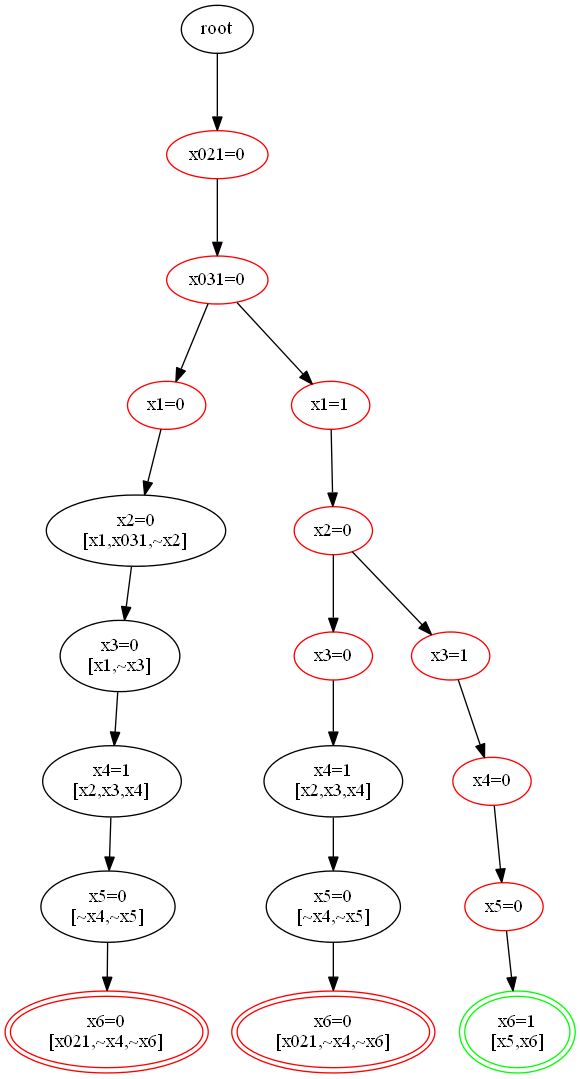
\includegraphics[keepaspectratio=true,height=.9\textheight]{tree1-color}
\end{center}
\caption{Tree of assignments for the DPLL algorithm}\label{tree1}
\end{figure}

Display option \p{tree\_inc} generates the trees incrementally whenever a conflict is reached.

%%%%%%%%%%%%%%%%%%%%%%%%%%%%%%%%%%%%%%%%%%%%%%%%%%%%%%%%%%%

\newpage

\section{Conflict-directed clause learning}

Select CDCL mode:
\begin{verbatim}
?- set_mode(cdcl).
\end{verbatim}

The display options relevant to this mode selected by default are:
\p{learned}, \p{resolvent}, \p{uip}.

After encountering the conflict clause \verb+[x5,x6]+, the algorithm \emph{learns} the clause \verb+[x021,~x4]+, as described in Sections~\ref{learned.dom}--\ref{learned.res}. When backtracking to assign 1 to \p{x3}, the learned clause becomes a unit clause based upon the previous assignment of 0 to \p{x021}. Unit propagation leads immediately to a satisfying assignment:

\begin{verbatim}
Conflict clause: [x5,x6]
  . . .
Learned clause from resolution (used): [x021,~x4]
Decision assignment: x1=1@3
Propagate unit: ~x4 (x4=0@3) derived from: [x021,~x4]
Decision assignment: x2=0@4
Propagate unit:  x3 (x3=1@4) derived from: [x2,x3,x4]
Decision assignment: x5=0@5
Propagate unit:  x6 (x6=1@5) derived from: [x5,x6]
Satisfying assignments:
[x021=0@1,x031=0@2,x1=1@3,x2=0@4,x3=1@4,x4=0@3,x5=0@5,x6=1@5]
Statistics: clauses=6, variables=8,
  units=8, decisions=6, conflicts=1, learned clauses=1
\end{verbatim}
Assignments are displayed together with their levels. Each decision
assignment increases the level, while assignments implied by unit
propagation receive the level of the last decision assignment. 

The search with CDCL is more efficient: compare the statistics (6
decisions and 1 conflict instead of 9 decisions and 2 conflicts) or the
the assignment trees (Figures~\ref{tree1}--\ref{tree2}).

\bigskip

For lookahead, occurrences of variables in the learned clauses are taken into account.

\begin{figure}
\begin{center}
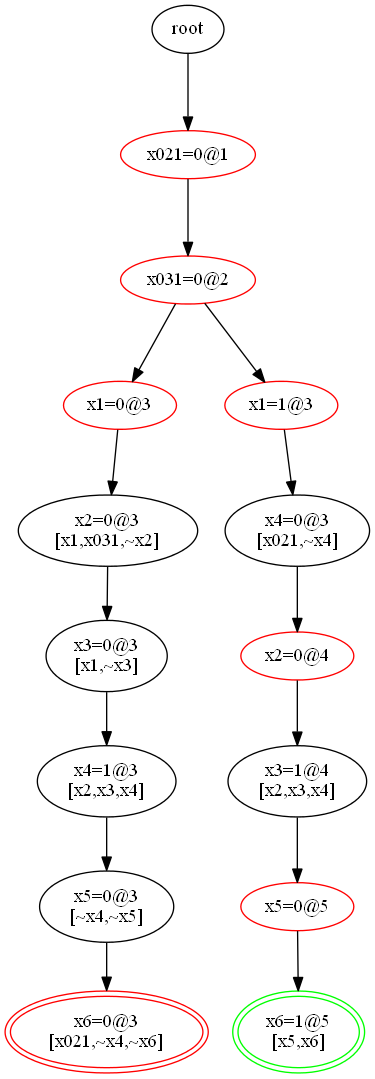
\includegraphics[keepaspectratio=true,height=.9\textheight]{tree2-color}
\end{center}
\caption{Tree of assignments for the DPLL algorithm with CDCL}\label{tree2}
\end{figure}

\clearpage

%%%%%%%%%%%%%%%%%%%%%%%%%%%%%%%%%%%%%%%%%%%%%%%%%%%%%%%%%%%


\section{The implication graph}

When a conflict clause is found, an \emph{implication graph} is
constructed and used to learn a clause.

\subsection*{Display options for generating a implication graph}

Display option \p{graph} displays a textual representation of the implication graph: a list of nodes and a list of edges.

\begin{verbatim}
Implication graph:
[kappa, x021=0@1, x031=0@2, x1=0@3, x2=0@3, x3=0@3, x4=1@3, x5=0@3, x6=0@3]
[
x021=0@1 --[x021,~x4,~x6]--> x6=0@3,
x031=0@2 --[x1,x031,~x2]--> x2=0@3,
x1=0@3 --[x1,x031,~x2]--> x2=0@3,
x1=0@3 --[x1,~x3]--> x3=0@3,
x2=0@3 --[x2,x3,x4]--> x4=1@3,
x3=0@3 --[x2,x3,x4]--> x4=1@3,
x4=1@3 --[~x4,~x5]--> x5=0@3,
x4=1@3 --[x021,~x4,~x6]--> x6=0@3,
x5=0@3 --[x5,x6]--> kappa,
x6=0@3 --[x5,x6]--> kappa
]
\end{verbatim}

Display option \p{dot} generates a \textsc{dot} representation of the graph and display option \p{label} causes the edges to be labeled with the antecedent clauses:

\begin{center}
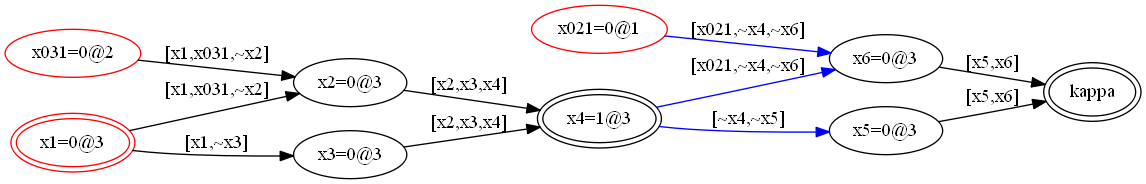
\includegraphics[keepaspectratio=true,width=\textwidth]{dom-color}
\end{center}

Display options \p{incremental} and \p{dot\_inc} generate the graphs after each step of the algorithm, not just when a conflict clause is reached.

\newpage

\subsection*{The meaning of an implication graph}

The implication graph represents the result of unit propagation that
leads to a conflict, starting from a set of decision assignments. In the
graph, are three source nodes, one for each of the decision assignments
(\p{x021=0@1}, \p{x031=0@2}, \p{x1=0@3}) that together lead to a
conflict by unit propagation.

The conflict is represented by the sink node \p{kappa} and the
assignments implied by unit propagation are represented by internal nodes labeled with the assignments. An edge of the graph is labeled with the
\emph{antecedent} clause of its target node. This is the unit clause
that implied the assignment labeling that node. For example, the
decision assignments \p{x1=0@3}, \p{x031=0@2} cause \verb+[x1,x031,~x2]+
to become a unit clause \verb+[~x2]+ and therefore this clause implies
the assignment of 0 to \p{x2}. The assignment receives the same level as
the last decision assignment so its node is labeled \p{x2=0@3}.

For each non-source node, there is an incoming edge for each literal in
the unit clause except the one whose assignment is implied. The
source nodes of these edges are the ones labeled with the assignments to
those literals. For example, the clause \verb+[x1,x031,~x2]+ with three
literals implied the assignment \p{x2=0@3}; therefore, the node labeled \p{x2=0@3} has two incoming edges: one from the node \p{x1=0@3} that assigned 0 to \p{x1} and one from the node \p{x031@2} that assigned 0 to \p{x031}.

The implication graph shows that the decision assignments \p{x021=0@1},
\p{x031=0@2}, \p{x1=0@3} cause a conflict. Clearly, if
\verb+[x021,x031,x1]+ were a clause in the original set of clauses, it
would be evaluated when the decisions were made. Since it evaluates to
0, it is a conflict clause that would be found immediately and there
would be no need to carry out unit propagation. Therefore, by
\emph{learning} this clause---adding it to our original set of
clauses---any subsequent decision assignments that include these three
would \emph{immediately} lead to the discovery of a conflict.

However, there is no advantage to learning a clause based only on decision assignments, because the same set of decisions at levels 1, 2 and 3 will never occur again after backtracking.

Sections~\ref{learned.dom}--\ref{learned.res} present algorithms that
can find \emph{shorter} learned clauses that are more likely to become
conflict clauses as the algorithm continues. Section~\ref{learned.dom}
describes how to learn a clause by computing a dominator in the
implication graph and Section~\ref{learned.res} describes how to learn a
clause resolving backwards from the conflict node.

The learned clause used by \ls{} is the one that is learned by resolution. The display options \p{learned}, \p{resolvent} and \p{uip} trace the computation by resolution. Display option \p{dominator} enables the computation and display of a dominator.

\newpage

%%%%%%%%%%%%%%%%%%%%%%%%%%%%%%%%%%%%%%%%%%%%%%%%%%%%%%%%%%%

\section{Learning a clause from a dominator}\label{learned.dom}

Here again is the implication graph:

\begin{center}
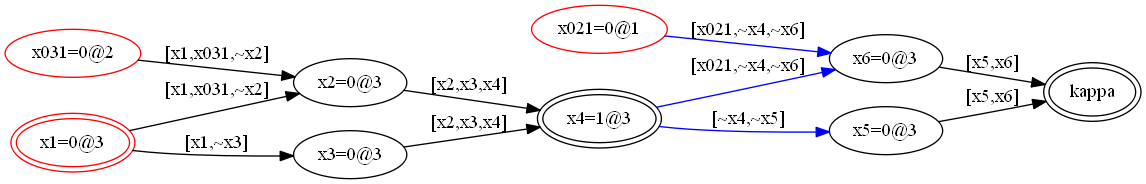
\includegraphics[keepaspectratio=true,width=\textwidth]{dom-color}
\end{center}

%\newpage

Consider all the (four) paths from the \emph{last} decision assignment, \p{x1=0@3}, the decision assignment at the highest level, to the node labeled \p{kappa}. The node \p{x4=1@3} is called a \emph{dominator} of a decision node if it appears on all the paths from the decision node to \p{kappa}. \ls{} computes the paths and finds a dominator:

\begin{verbatim}
Paths from the decision node at this level to kappa:
x1=0@3 --> x2=0@3 --> x4=1@3 --> x5=0@3 --> kappa
x1=0@3 --> x2=0@3 --> x4=1@3 --> x6=0@3 --> kappa
x1=0@3 --> x3=0@3 --> x4=1@3 --> x5=0@3 --> kappa
x1=0@3 --> x3=0@3 --> x4=1@3 --> x6=0@3 --> kappa
A dominator is: x4=1@3
\end{verbatim}

A dominator is a \emph{unique implication point (UIP)} because its
assignment participates in the conflict in the same way as do \emph{all}
the decision assignments that it dominates. Here, the assignment
\p{x4=1@3} is implied by the \emph{two} assignments \p{x031=0@2} and
\p{x1=0@3}, so \verb+~x4+ can replace \p{x031} and \p{x1} in the learned
clause \verb+[x021,x031,x1]+ to obtain a shorter learned clause
\verb+[x021,~x4]+.

There remains one path from a decision node to \p{kappa} that does not
contain the dominator:
\begin{verbatim}
Paths from decision nodes at lower levels to kappa:
x021=0@1 --> x6=0@3 --> kappa
\end{verbatim}

The learned clause is therefore composed of the complement of the
assignment at the UIP, together with the complements of assignments at
\emph{higher} levels that are not dominated by the UIP. The literal
chosen for this path is the one just before the path joins an assignment
at the lowest level; in this case, it is the decision assignment to
\verb+x021+:

\begin{verbatim}
Learned clause from dominator (not used): [x021,~x4]
\end{verbatim}

The blue lines form a \emph{cut}: their source nodes are the
assignments that define the literals in the learned clause. These nodes
define a learned clause because assignments to the literals necessarily
lead to the conflict. The cut we chose includes the edges whose source
node is the UIP together with an edge on each path from a decision node
that is not dominated by the UIP.

\newpage

%%%%%%%%%%%%%%%%%%%%%%%%%%%%%%%%%%%%%%%%%%%%%%%%%%%%%%%%%%%

\section{Learning a clause by resolution}\label{learned.res}

The learned clause can be obtained by resolution starting with the
conflict clause---the antecedent clause of the \p{kappa} node---and
terminating when a UIP is found. The conflict clause as the
initial \emph{current clause}. At each step, the antecedent clause at clashes with the current clause on the literal that was
assigned at that node by unit propagation. For example, given the
initial current clause \verb+[x5,x6]+, the conflict resulted from the assignment of 0 to \p{x5} which was forced by the assignment of 1 to \verb+~x5+, the literal in the unit clause \verb+[~x4,~x5]+. The two clauses have clashing literals, so we can resolve \verb+[x5,x6]+ with the \verb+[~x4,~x5]+ to obtain the resolvent \verb+[~x4,x6]+ which becomes the new current clause.

The next step is to resolve this clause with \verb+[x021,~x4,~x6]+, the antecedent of the assignment to \p{x6}, to obtain \verb+[x021,~x4]+. The resolution now terminates because this clause is associated with a UIP: there is one (implied) literal assigned at the current level and the other literals were assigned by decision assignments at higher levels.

Here is the computation as displayed by \ls{}:
\begin{verbatim}
Conflict clause: [x5,x6]
Not a UIP: two literals [x6,x5] are assigned at level: 3
Resolvent: of [x5,x6] and antecedent [x021,~x4,~x6] is [x5,x021,~x4]
Not a UIP: two literals [~x4,x5] are assigned at level: 3
Resolvent: of [x5,x021,~x4] and antecedent [~x4,~x5] is [x021,~x4]
UIP: one literal ~x4 is assigned at level: 3
Learned clause from resolution (used): [x021,~x4]
\end{verbatim}

Since the conflict clause is unsatisfiable under the current set of
decision assignments, so is the set consisting of it and its clashing
clause, and therefore their resolvent---the next current clause---is
also unsatisfiable.

For example, \verb+[x5,x6]+ is a conflict clause because it evaluates to
0. The antecedent clause \verb+[~x4,~x5]+ is a unit clause and therefore
exactly one literal is assigned 1. Since both literals in the conflict
clause \verb+[x5,x6]+, are assigned 0, \verb+~x5+, the complement of
\verb+x5+, is assigned 1, so it must be the \emph{only} literal in the
antecedent clause \verb+[~x4,~x5]+ that is assigned 1. Therefore,
\verb+~x4+ is assigned 0 and we conclude that all literals in the
resolvent \verb+[~x4,x6]+ are assigned 0.

Which of these clauses should we learn? Successive resolution steps will
eventually lead back to the clause defined by the decision nodes
(\verb+[x021,x031,x1]+), but there is no advantage to learning this
clause. However, the resolvent clause associated with a UIP
(\verb+[x021,~x4]+) contains only a single literal at the current level
(\verb+~x4+), so it can replace the decision literal at the same level
(\verb+x1+), as well as any decision variables at higher levels that are
dominated by the UIP (\verb+x031+).

\newpage
%%%%%%%%%%%%%%%%%%%%%%%%%%%%%%%%%%%%%%%%%%%%%%%%%%%%%%%%%%%

\section{Non-chronological backtracking}

Select NCB mode:
\begin{verbatim}
?- set_mode(ncb).
\end{verbatim}

When a learned clause has been obtained, the backtrack level for
non-chronological backtracking is computed. This is the highest level of
an assignment in the learned clause except for the current level. In the
example, the learned clause is \verb+[x021,~x4]+, where \p{x4} was
assigned at level 3, the current level, and \p{x021} was assigned at
level 1, which becomes the backtrack level. When backtracking, we can
skip decision assignments whose level is at a higher level than the
backtrack level, in the example, the decision assignments at levels 3
and 2:

\begin{verbatim}
Non-chronological backtracking to level: 1
Skip decision assignment: x1=1@3
Skip decision assignment: x031=1@2
\end{verbatim}

Once 0 is assigned to \p{x021} at level 1, the clause \verb+[x021,~x4]+
becomes a unit clause \verb+[~x4]+ which forces the assignment of 0 to
\p{x4}. Consider now the original set of clauses:

\begin{verbatim}
[[x1,x031,~x2], [x1,~x3], [x2,x3,x4], [~x4,~x5], [x021,~x4,~x6], [x5,x6]]
\end{verbatim}
Under these two assignments, the set becomes:
\begin{verbatim}
[[x1,x031,~x2], [x1,~x3], [x2,x3], [x5,x6]]
\end{verbatim}
The next decision assignment was 0 to \p{x031} giving:
\begin{verbatim}
[[x1,~x2], [x1,~x3], [x2,x3], [x5,x6]]
\end{verbatim}

If 0 is assigned to \p{x1}, \p{[x2,x3]} becomes a conflict clause. It
follows that 1 must be assigned to \p{x1} and there is no need to
\emph{flip} the variable (assign the other Boolean value to the
variable); therefore, we can skip over \p{x1} when backtracking.

Once we know that 1 is assigned to \p{x1}, the clause
\verb+[x1,x031,~x2]+ becomes true and can be deleted. Since that clause
contains the only occurrence of the variable \p{x031}, it follows that if
there exists a satisfying assignment, it is independent of the value
assigned to \p{x031}, so, again, we can skip over \p{x031} when
backtracking.

From the learned clause, it follows that \emph{the assignment of 0
to \p{x021} by itself makes it unnecessary to flip the variables
\p{x031} and \p{x1}}. We can backtrack directly to flip the variable
\p{x021}.

NCB can be seen in the tree of assignments (Figure~\ref{tree3}). The
graph is no longer a tree but a DAG (directed acyclic graph) because
once \p{x021} is assigned (0 or 1), the assignments of 0 to \p{x031} and
then \p{x1} lead to the same sequence of unit propagations. The graph
branches only at its leaves because one assignment leads to a conflict
clause and the other to a satisfying assignment.

\begin{figure}
\begin{center}
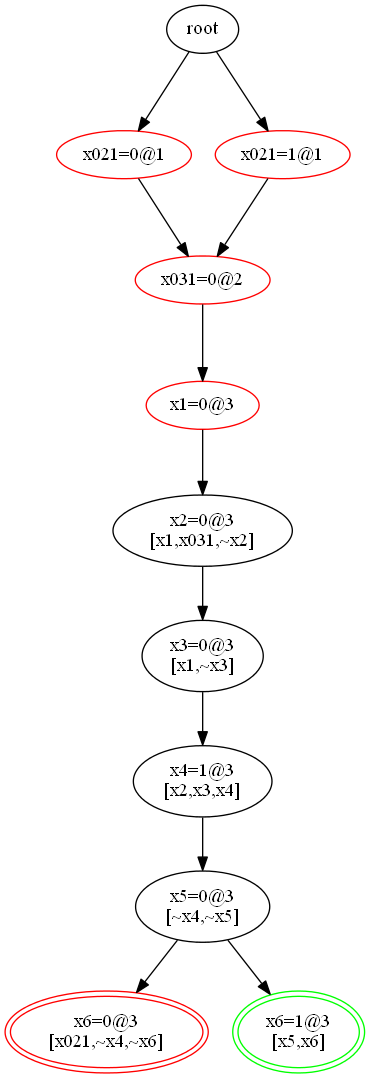
\includegraphics[keepaspectratio=true,height=.9\textheight]{tree3-color}
\end{center}
\caption{Tree of assignments for the DPLL algorithm with CDCL and NCB}\label{tree3}
\end{figure}

\clearpage

%%%%%%%%%%%%%%%%%%%%%%%%%%%%%%%%%%%%%%%%%%%%%%%%%%%%%%%%%%%
%%%%%%%%%%%%%%%%%%%%%%%%%%%%%%%%%%%%%%%%%%%%%%%%%%%%%%%%%%%

\chapter{Combinatorics, numbers, graphs}\label{ch.comb}

Problems from combinatorics are a rich source of examples for SAT solving. The chapter starts with the well-known pigeonhole principle, which is examined in detail. This is followed by the classic $n$-queens problem and the solution of Sudoku puzzles. Four problems from number theory follow: Ramsey theory, Schur triples, Langford's problem and van der Waerden's problem. These were inspired by the presentations in \cite{brute,knuth-sat}. The next two problems are more complex: pebbling problems and seating guests at a table under constraints. SAT solvers can be used on graphs. In Section~\ref{s.graph-color}, we show how a complex planar graph can be colored using four colors. The existence of such a coloring following from the Four Color Theorem that was proved relative recently. Section~\ref{s.color-queens} gives a variant of the $n$-queens problem: can you placed colored queens on every square such that no row, column and diagonal contains queens of the same color. Section~\ref{s.tseitin} presents Tseitin graphs that used studies for resolution.



\section{The pigeonhole principle}\label{ch.pigeon}

\fl{pigeon.pro}

The pigeonhole principle states that if we place $n+1$ pigeons in $n$
holes then one hole contains at least two pigeons. Therefore, a formula
stating that all pigeons are in different holes must be unsatisfiable.
Let \p{pij} be an atom whose intended meaning is that pigeon \p{i} is in
hole \p{j}; for two holes and three pigeons, the set of clauses is:

\begin{verbatim}
  [p11, p12],   [p21, p22],   [p31, p32],   % Each pigeon in hole 1 or 2 
  [~p11, ~p21], [~p11, ~p31], [~p21, ~p31], % No pair is in hole 1
  [~p12, ~p22], [~p12, ~p32], [~p22, ~p32], % No pair is in hole 2
\end{verbatim}

\newpage

For three holes and four pigeons the formula is:

\begin{verbatim}
  % Each pigeon in at least hole
  [p11, p12, p13], [p21, p22, p23], [p31, p32, p33], [p41, p42, p43], 
  % Each hole has at most one pigeon
  [~p11, ~p21], [~p11, ~p31], [~p11, ~p41],
  [~p21, ~p31], [~p21, ~p41], [~p31, ~p41],
  [~p12, ~p22], [~p12, ~p32], [~p12, ~p42],
  [~p22, ~p32], [~p22, ~p42], [~p32, ~p42],
  [~p13, ~p23], [~p13, ~p33], [~p13, ~p43],
  [~p23, ~p33], [~p23, ~p43], [~p33, ~p43]
\end{verbatim}

For the two-hole formula, the mode chosen makes no difference, but for
the three-hole formula, NCB makes a significant improvement:

\begin{verbatim}
dpll: units=49, decisions=16, conflicts=9
cdcl: units=42, decisions=16, conflicts=9, learned clauses=6
ncb:  units=25, decisions=10, conflicts=3, learned clauses=3
\end{verbatim}

If you look at the trace in NCB mode, the following clauses are
learned:

\begin{verbatim}
[p43,p33,~p22],   [p42,p32,~p23],  [p41,p31,~p23]
\end{verbatim}

Six decision assignments are skipped---both 0 and 1 for the variables
\p{p12}, \p{p13} and \p{p22}---so there are only three conflict instead
of nine.

Let us look now at the implication graphs. The graph for the two-hole
formula is shown in Figure~\ref{pigeon2} (shown top-to-bottom instead of
left-to-right). The conflict clause is \verb+[~p12,~p32]+ (stating
that either pigeon~1 or pigeon~3 is not in hole 2) and the
dominator is the node labeled \verb+p12=1@1+. Since \emph{all} nodes
are assigned at level~1, by resolving backwards we should be able to
learn the (unit) clause \verb+[~p12]+.

\begin{figure}
\begin{center}
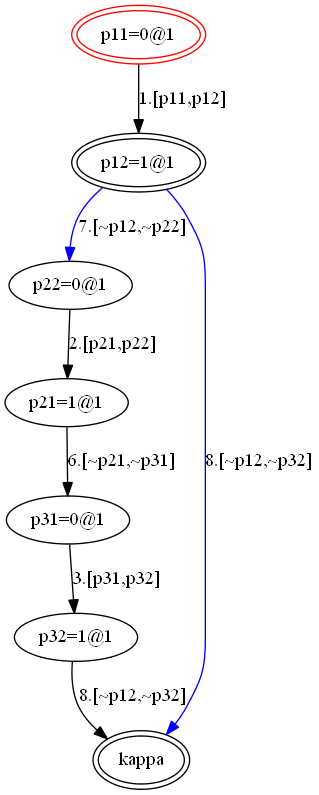
\includegraphics[keepaspectratio=true,height=.9\textheight]{pigeon2-color}
\end{center}
\caption{Implication graph for two-hole pigeonhole}\label{pigeon2}
\end{figure}

However, we must be careful. According to \cite[p.~137]{mlm}: ``at each
step $i$, a literal $l$ assigned at the current decision level $d$ is
selected and the intermediate clause (\ldots) is resolved with the
antecedent of $l$.'' If we \emph{select} \verb+~p12+ and resolve \verb+[~p12,~p32]+ with \verb+[p11,p12]+, the antecedent of the second node from the top, the result is \verb+[p11,~p32]+, which is actually worse than just taking
the decision node \verb+[p11]+. When selecting the literal to resolve,
we must be careful to choose the \emph{last} one that was assigned, here
\verb+~p32+. If this is done, the sequence of resolvents is:

\newpage

\begin{verbatim}
Conflict clause: [~p12,~p32]
Resolvent: of [~p12,~p32] and antecedent [p31,p32] is [~p12,p31]
Resolvent: of [~p12,p31] and antecedent [~p21,~p31] is [~p12,~p21]
Resolvent: of [~p12,~p21] and antecedent [p21,p22] is [~p12,p22]
Resolvent: of [~p12,p22] and antecedent [~p12,~p22] is [~p12]
UIP: one literal ~p12 is assigned at level: 1
Learned clause from resolution: [~p12]
\end{verbatim}

The implication graph for the three-hole formula is shown in
Figure~\ref{pigeon3}. The node labeled \verb+p22=1@3+ is a dominator and
the clause learned by resolution is \verb+[p43,p33,~p22]+. The blue
lines shows the \emph{cut}: it is sufficient to assign to the three
literals before the cut in order to obtain a conflict, and the
complements of these literals form the learned clause.

The literals that form part of the learned clause come from assignments
at higher levels that are \emph{not} decision assignments, but
assignments implied by unit propagation: \verb+p43+ and \verb+p33+ which
are assigned at level~2.

\begin{figure}
\begin{center}
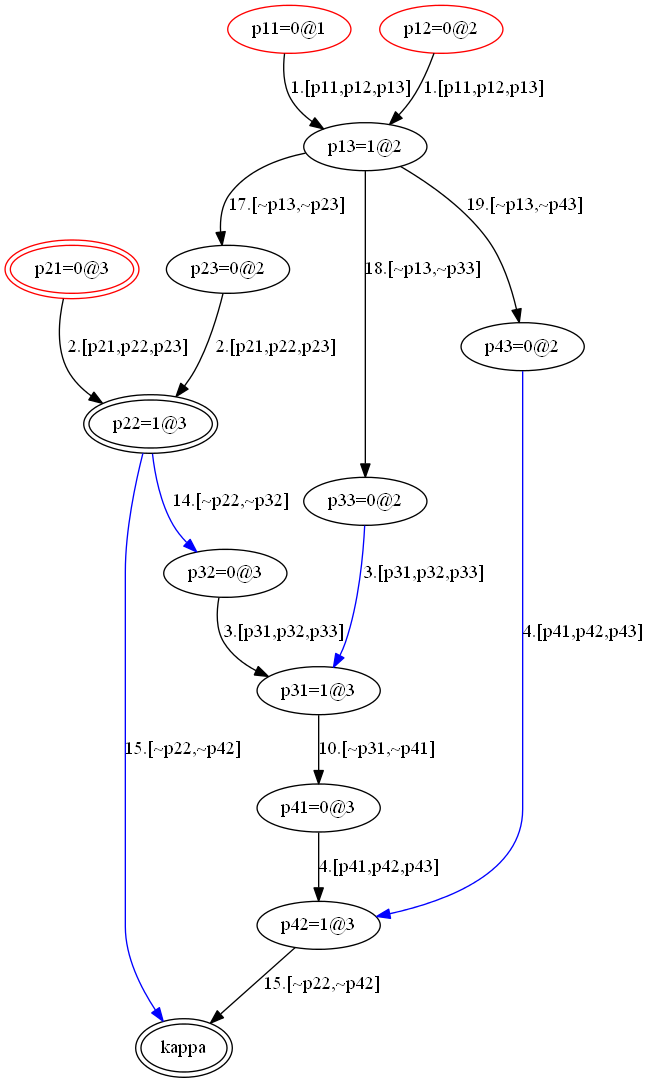
\includegraphics[keepaspectratio=true,height=.9\textheight]{pigeon3-color}
\end{center}
\caption{Implication graph for three-hole pigeonhole}\label{pigeon3}
\end{figure}

\clearpage
%%%%%%%%%%%%%%%%%%%%%%%%%%%%%%%%%%%%%%%%%%%%%%%%%%%%%%%%%%%

\section{The $n$-queens problem}\label{ch.queens}

\fl{queens.pro}

The $n$-queens problem is to place $n$ queens on an $n \times n$ chess
board such that no queen can capture another. The archive includes programs for both $4$ queens and $8$ queens. Here we look at a $4\times 4$ board. A solution is:

\begin{center}
\unitlength=1.0pt
\begin{picture}(100,100)
\put(0,0){
  \multiputlist(20,0)(20,0){1,2,3,4}
  \multiputlist(0,20)(0,20){4,3,2,1}
}
\put(10,10){
  \put(0,0){\grid(80,80)(20,20)}
  \put( 0, 20){\makebox(20,20){Q}}
  \put(20, 60){\makebox(20,20){Q}}
  \put(40,  0){\makebox(20,20){Q}}
  \put(60, 40){\makebox(20,20){Q}}
}
\end{picture}
\end{center}

The problem can be encoded in clausal form using 80 clauses on 16
variables \cite[Section~6.4]{mlcs}. Other encodings are discussed in
\cite[Section 2.3.1]{cnf} based on \cite{nadel}. The 4-queens problem
has a solution (in fact, two solutions), so the formula will be
satisfiable and the satisfying assignments provide a solution:

\begin{verbatim}
[p11=0,p12=0,p13=1,p14=0,p21=1,p22=0,p23=0,p24=0,
 p31=0,p32=0,p33=0,p34=1,p41=0,p42=1,p43=0,p44=0]
\end{verbatim}
where \p{pij} is true if a queen is placed in column \p{i} and row \p{j}. 

The statistics for the different modes are:
\begin{verbatim}
dpll: units=30, decisions=6, conflicts=2
cdcd: units=30, decisions=6, conflicts=2, learned clauses=2
ncb:  units=25, decisions=5, conflicts=1, learned clauses=1
\end{verbatim}

If you examine the assignment tree for the DPLL algorithm (not shown),
you will see the effectiveness of unit propagation. Just three decision
assignments (\p{p11=0@1}, \p{p12=0@2}, \p{p13=0@3}) imply the assignment
\p{p14=1@3}, which in turn implies more assignments of 0 along its row and
diagonal. The placement of the first queen is shown on the left of
Figure~\ref{queens}, where the subscripts denote the assignment level and
primes denote the inferred assignments.

\begin{figure}[tb]
\begin{center}
\begin{tabular}{l@{\hspace{.2\textwidth}}r}
\unitlength=1.0pt
\begin{picture}(100,100)
\put(0,0){
  \multiputlist(20,0)(20,0){1,2,3,4}
  \multiputlist(0,20)(0,20){4,3,2,1}
}
\put(10,10){
  \put(0,0){\grid(80,80)(20,20)}
  \put( 0, 20){\makebox(20,20){$0_3$}}
  \put( 0, 40){\makebox(20,20){$0_2$}}
  \put( 0, 60){\makebox(20,20){$0_1$}}
  \put( 0, 0){\makebox(20,20){$1'_3$}}
  \put(20, 0){\makebox(20,20){$0'_3$}}
  \put(40, 0){\makebox(20,20){$0'_3$}}
  \put(60, 0){\makebox(20,20){$0'_3$}}
  \put(20,20){\makebox(20,20){$0'_3$}}
  \put(40,40){\makebox(20,20){$0'_3$}}
  \put(60,60){\makebox(20,20){$0'_3$}}
}
\end{picture}
&
\begin{picture}(100,100)
\put(0,0){
  \multiputlist(20,0)(20,0){1,2,3,4}
  \multiputlist(0,20)(0,20){4,3,2,1}
}
\put(10,10){
  \put(0,0){\grid(80,80)(20,20)}
  \put( 0, 20){\makebox(20,20){$0_3$}}
  \put( 0, 40){\makebox(20,20){$0_2$}}
  \put( 0, 60){\makebox(20,20){$0_1$}}
  \put( 0, 0){\makebox(20,20){$1'_3$}}
  \put(20, 0){\makebox(20,20){$0'_3$}}
  \put(40, 0){\makebox(20,20){$0'_3$}}
  \put(60, 0){\makebox(20,20){$0'_3$}}
  \put(20,20){\makebox(20,20){$0'_3$}}
  \put(40,40){\makebox(20,20){$0'_3$}}
  \put(60,60){\makebox(20,20){$0'_3$}}
  \put(20,60){\makebox(20,20){$0_4$}}
  \put(20,40){\makebox(20,20){$1'_4$}}
  \put(60,40){\makebox(20,20){$0'_4$}}
  \put(60,20){\makebox(20,20){$1'_4$}}
  \put(40,20){\makebox(20,20){$0'_4$}}
  \put(40,60){\makebox(20,20){$1'_4$}}
}
\end{picture}
\end{tabular}
\caption{Decisions and implications for the four-queens
problem}\label{queens}
\end{center}
\end{figure}

The next decision assignment is \p{p21=0@4} or \p{p21=1@4}, both of
which lead to conflicts. Let us look at \p{p21=0@4}. \p{p21=0@4} implies
\p{p22=1@4} because there has to be a queen in the second column. The
next implications are \p{p42=0@4}, \p{p43=1@4}, \p{p33=0@4}, \p{p31=1@4}
(see the right of Figure~\ref{queens}). Clearly, there is a conflict
because the clause \verb+[~p22,~p31]+ is false. The intended meaning of
this clause is that either there is no queen in (column 2, row 2) or
there is no queen in (column 3, row 1) because they can capture each
other.

We leave it to the reader to examine the sequence of assignments
following the decision assignment \p{p21=1@4} and to show that it too
leads to a conflict.

Figure~\ref{queens-ig} shows the implication graph with the dominator
node \verb+p22=1@4+ and the cut that defines the learned clause
\verb+[~p22,p32,p34,p41,p44]+. The learned clause is such that the
decision assignments at the higher levels (\verb+p11=0@1+,
\verb+p12=0@2+, \verb+p13=0@3+) make it a unit clause \verb+[~p22]+ and
force the assignment \p{p22=1@4}, regardless of the assignment to
\p{p21}. Therefore, non-chronological backtracking can skip the
assignment \p{p21=1@4} and continue with the previous decision
assignment. The assignment \p{p13=1@3} instead of \p{p13=0@3} leads to a
satisfying assignment by unit propagation alone!
 
\begin{figure}[b]
\begin{center}
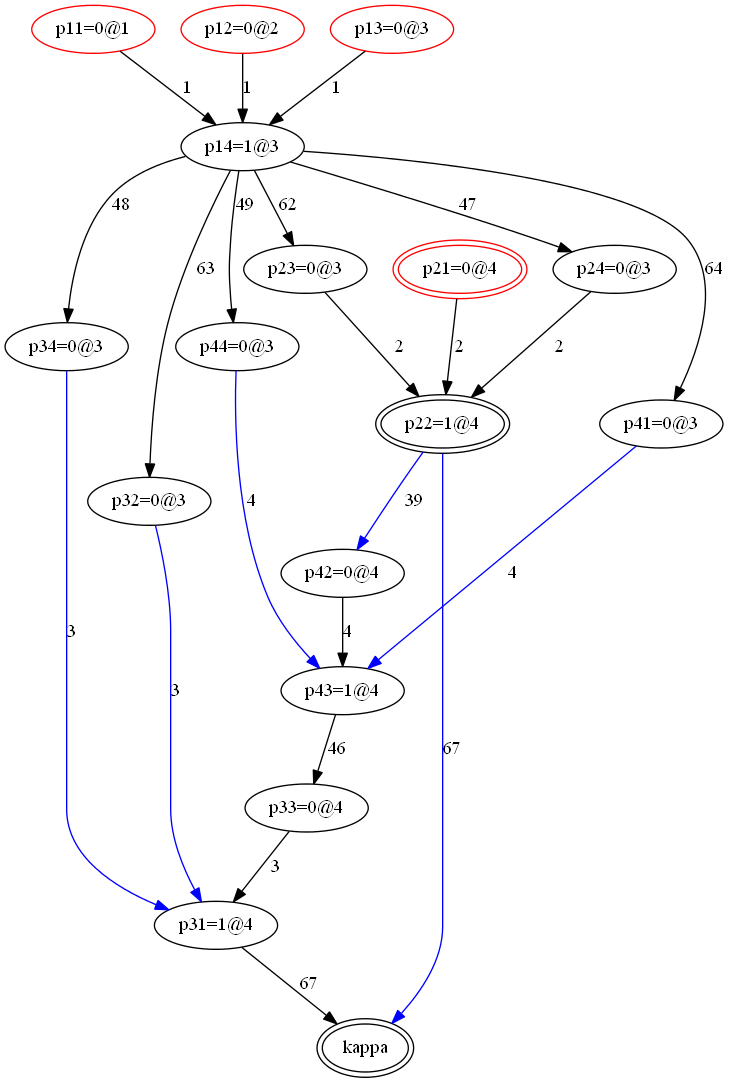
\includegraphics[keepaspectratio=true,height=.8\textheight]{queens-color}
\end{center}
\caption{Implication graph for the four-queens}\label{queens-ig}
\end{figure}


%%%%%%%%%%%%%%%%%%%%%%%%%%%%%%%%%%%%%%%%%%%%%%%%%%%%%%%%%%%

\section{Sudoku}

\fl{sudoku.pro}

The encoding of an $n\times n$ Sudoku puzzle into CNF is straightforward but requires quite a few clauses. You need clauses to express that each of the $n$ numbers appear in each row, column and block, and that no number appears twice. The archive includes two CNF formulas for a $4\times 4$ Sudoku puzzle: one with the full CNF and one with a simpler CNF. The simpler CNF does not include that clauses specifying that no number appear twice in each row, column and block, because if all $n$ numbers appear once, than none appears twice. You can experiment to determine which encoding is more efficient.

The CNF formulas were generated using a program by Ivor Spence that outputs DIMACS, which was converted to the \ls{} CNF format using the program \p{dimacs.pro}.\\
See: \url{http://www.cs.qub.ac.uk/~I.Spence/SuDoku/SuDoku.html}.

\clearpage

%%%%%%%%%%%%%%%%%%%%%%%%%%%%%%%%%%%%%%%%%%%%%%%%%%%%%%%%%%%

\section{Ramsey numbers}

\fl{ramsey.pro}

Ramsey's Theorem states that for any $n$, there is a smallest number $R(n)$ with the following property: If the edges of the complete graph on $R(n)$ vertices are colored with two colors then there must be a monochromatic complete subgraph with $n$ vertices. The archive contains CNF formulas that show that $R(3)>5$ and $R(3) = 6$. The following drawing shows that it is possible to color $K_5$ with two colors such that there is no monochromatic triangle.

% The following diagram was generated using TikZ
% You can find the source in the file tikz.tex

\begin{center}
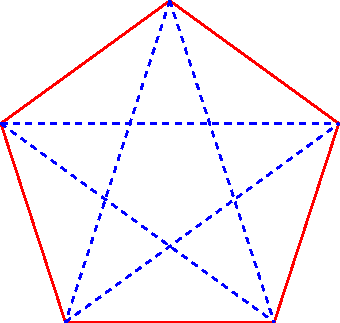
\includegraphics{ramsey.pdf}
\end{center}

The CNF encoding uses \p{true} for one color and \p{false} for the other. For each of the ten triangles in $K_5$, there is a pair of clauses that ensure that at least one edge is colored \p{true} and one \p{false}:
\begin{verbatim}
  [x12,x23,x13], [~x12,~x23,~x13],
\end{verbatim}
The set of clauses is satisfiable.

For $K_6$, there is pair of clauses for each of the nineteen triangles. The formula is unsatisfiable, meaning that it is not true that there exists a triangle that is not monochromatic, that is, there must be a monochromatic triangle. Therefore, $R(3) = 6$.
	
%%%%%%%%%%%%%%%%%%%%%%%%%%%%%%%%%%%%%%%%%%%%%%%%%%%%%%%%%%%

\section{Schur triples}

\fl{schur.pro}

Given \emph{any} decomposition of the natural numbers $S=\{1,\ldots,n\}$ into two mutually exclusive subsets $S_1,S_2$, do there exist $a,b,c\in S_i$, $a<b<c$, $a+b=c$, for at least one $i=1,2$? The set of numbers $\{a,b,c\}$ is called a \emph{Schur triple}. For $n=8$, there are decompositions with no triples:
\[
S_1 = \{1,2,4,8\}, S_2 = \{3,5,6,7\}.
\]
The archive contains CNF formulas showing that for $n=8$, there are decompositions with no Schur triples, but for $n=9$, all decompositions contain a Schur triple. If equality is allowed $a\leq b$, the numbers are $n=4$ and $n=5$, respectively.

The encoding is similar to that used for Ramsey numbers with \p{true} representing one set and \p{false} representing the other set. For each $\{a,b,c\}$ such that $a+b=c$, the following pair of clauses states that at least one of $x_a,x_b,x_c$ must be \p{true} and at least one must be \p{false}:
\begin{verbatim}
  [x3,x4,x7], [~x3,~x4,~x7],
\end{verbatim}
For $n=8$ the formula is satifiable, but for $n=9$ it is unsatisfiable.

%%%%%%%%%%%%%%%%%%%%%%%%%%%%%%%%%%%%%%%%%%%%%%%%%%%%%%%%%%%

\section{Langford's problem}

\fl{generate-langford.pro, langford.pro}

Langford's problem $L(n)$ asks if it is possible to arrange pairs of numbers $1,1,2,2,3,3,\ldots,n,n$ in a sequence so the two occurrences of each number $k$ are separated by $k$ other numbers. It is easy to see that $312132$ is a solution for $n=3$ and $41312432$ is a solution for $n=4$. Here we show how to solve $L(3)$ and $L(4)$ using SAT solving. The presentation is based on \cite{knuth-sat}; for more information on Langford's problem see \cite{miller-lang}.

The problem can be posed using an array. For $n=3$, there are $6$ columns, one for each of the $2n$ numbers. The rows represent the specification of the problem: the occurrences of $k$ must have $k$ numbers between them. It is easy to see that there are four possible placements of $1$, three of $2$ and two of $3$:

\begin{center}
\begin{tabular}{|c||c|c|c|c|c|c|}
\hline
&1&2&3&4&5&6\\\hline\hline
1&1&&1&&&\\\hline
2&&1&&1&&\\\hline
3&&&1&&1&\\\hline
4&&&&1&&1\\\hline
5&2&&&2&&\\\hline
6&&2&&&2&\\\hline
7&&&2&&&2\\\hline
8&3&&&&3&\\\hline
9&&3&&&&3\\\hline
\end{tabular}
\end{center}

To solve the problem, we need to select \emph{one} row for the positions of the $1$'s in the sequence, \emph{one} row for the $2$'s and \emph{one} row for the $3$'s, such that if we stack just these rows on top of each other, no column contains more than one number:

\begin{center}
\begin{tabular}{|c||c|c|c|c|c|c|}
\hline
&1&2&3&4&5&6\\\hline\hline
2&&1&&1&&\\\hline
7&&&2&&&2\\\hline
8&3&&&&3&\\\hline
\end{tabular}
\end{center}

First, note that row 9 is not needed because of symmetry: starting with row 9 just gives the reversal of the  sequence obtained by starting with row 8.

Row 8 is the only one containing $3$'s so it must be chosen and the result is 3\textvisiblespace \textvisiblespace \textvisiblespace 3\textvisiblespace. Any row with numbers in columns 1 and 5 can no longer be used, because only one number can be placed at each position: $\not 1,2,\not 3,4,\not 5, \not 6, 7, 8$.

Row 7 is the only remaining row containing $2$'s so must be chosen and the result is 3\textvisiblespace 2\textvisiblespace 3{}2. Deleting rows that can no longer be used gives: $\not 1,2,\not 3,\not 4,\not 5, \not 6, 7, 8$.

Choosing the only remaining row, row 2, gives 3{}1{}2{}1{}3{}2.

Let us encode Langford's problem. Let $x_i$ be true if row $i$ is chosen. The following clauses encode that exactly one of rows 1,2,3,4 must be chosen:
\begin{verbatim}
  [x1,x2,x3,x4],
  [~x1,~x2], [~x1,~x3], [~x1,~x4],
  [~x2,~x3], [~x2,~x4],
  [~x3,~x4]
\end{verbatim}
The first clause encodes that at least one of these rows must be chosen and the other clauses encode at most one of the rows can be chosen. There are similar sets of clauses for rows 5, 6, 7, and for row 8 (which is a unit clause because there are no alternatives).

In the same way, we encode clauses expressing the constraints on the columns. For example, column 1 requires that exactly one of rows 1, 5, 8 be chosen:
\begin{verbatim}
  [x1,x5,x8], [~x1,~x5], [~x1,~x8], [~x5,~x8]
\end{verbatim}

For $n=3$ there are 32 clauses on the 8 variables, and the DPLL algorithms finds the solution immediately using just unit propagation starting with \texttt{x8}.

The archive contains a set of clauses $L(4)$. Running DPLL gives:
\begin{verbatim}
clauses=101, variables=17, units=50, decisions=10, conflicts=4
\end{verbatim}
The reader is encouraged to check if \texttt{cdcl}, \texttt{ncb} or \texttt{look} can improve the performance.

\newpage

%%%%%%%%%%%%%%%%%%%%%%%%%%%%%%%%%%%%%%%%%%%%%%%%%%%%%%%%%%%

\section{van der Waerden's problem}

\fl{generate-vdw.pro, vdw.pro}

Consider two sequences of eight binary digits:
\[
00011100,\; 01010011,\; 00110011\,.
\]
The first sequence has a subsequence of three consecutive $0$'s, as well as a one of three consecutive $1$'s. The second sequence has three $0$'s two positions away from each other: the digits at position $1$ (counting from the left), position $3$ and position $5$. The third sequence has \emph{no} subsequence of three equal digits that equally spaced from each other. If you try to find a sequence of \emph{nine} binary digits with no subsequence of equally spaced digits, you will not succeed. For example, adding a $0$ to the end of the third sequence above gives $001100110$ and there is a subsequence of $0$'s at positions $1,5,9$, and if add a $1$, the sequence $001100111$ has three consecutive $1$'s at the end.

van der Waerden's problem for $k$ asks what is the smallest number $n$ such that any sequence of $n$ digits contains $k$ equally spaced digits.

To solve van der Waerden's problem with a SAT solver, use an encoding similar to the encoding of Schur triples. For $n=8$ the encoding is:
\begin{verbatim}
  [x1,x2,x3],[~x1,~x2,~x3],
  [x2,x3,x4],[~x2,~x3,~x4],
  [x3,x4,x5],[~x3,~x4,~x5],
  [x4,x5,x6],[~x4,~x5,~x6],
  [x5,x6,x7],[~x5,~x6,~x7],
  [x6,x7,x8],[~x6,~x7,~x8],
  [x1,x3,x5],[~x1,~x3,~x5],
  [x2,x4,x6],[~x2,~x4,~x6],
  [x3,x5,x7],[~x3,~x5,~x7],
  [x4,x6,x8],[~x4,~x6,~x8],
  [x1,x4,x7],[~x1,~x4,~x7],
  [x2,x5,x8],[~x2,~x5,~x8]
\end{verbatim}
This formula is satisfiable:
\begin{verbatim}
Satisfying assignments: [x1=0,x2=0,x3=1,x4=1,x5=0,x6=0,x7=1,x8=1]
\end{verbatim}
and corresponds to the sequence $00110011$ which has no equally spaced subsequence of length three. We can extending the encoding for sequences of length $n=9$ by adding the clauses:
\begin{verbatim}
  [x7,x8,x9],[~x7,~x8,~x9],
  [x5,x7,x9],[~x5,~x7,~x9],
  [x3,x6,x9],[~x3,~x6,~x9],
  [x1,x5,x9],[~x1,~x5,~x9]
\end{verbatim}
\ls{} now returns that the formula is unsatisfiable, meaning that there is no sequence without an equally spaced subsequence of length three.

The archive contains formulas that show that there are sequences of length $n=34$ with no equally spaced subsequences of length four, but that is not possible for sequences of length $n=35$. All formulas were generated by the program \p{generate-vdw.pro}.

%%%%%%%%%%%%%%%%%%%%%%%%%%%%%%%%%%%%%%%%%%%%%%%%%%%%%%%%%%%

\section{Pebbling formulas}

\fl{pebbling.pro}

A pebbling formula represents the scheduling of tasks. Each task is
represented by a node in a directed acylic graph. In the following
diagram the task represented by the topmost node can be performed by
``machine'' $p_1$ \emph{or} by ``machine'' $p_2$; however, it can begin
only when both of the two tasks below it have been completed. In turn,
each of those tasks can be performed by one of two machines and can
begin only after the previous tasks at the source of its incoming edges
have been completed.

\begin{center}
\begin{picture}(193,105)
%\put(0,0){\framebox(193,105){}}
\put(0,0){
\multiput(20,20)(76,0){3}{\circle*{4}}
\put(10,0){\makebox(20,20){$s_1 \vee s_2$}}
\put(86,0){\makebox(20,20){$t_1 \vee t_2$}}
\put(162,0){\makebox(20,20){$u_1 \vee u_2$}}
\put(22,22){\vector(1,1){32}}
\put(94,22){\vector(-1,1){32}}
\put(98,22){\vector(1,1){32}}
\put(170,22){\vector(-1,1){32}}
}
\put(38,36){
\multiput(20,20)(76,0){2}{\circle*{4}}
\put(-15,12){\makebox(20,20){$q_1 \vee q_2$}}
\put(110,12){\makebox(20,20){$r_1 \vee r_2$}}
\put(22,22){\vector(1,1){32}}
\put(94,22){\vector(-1,1){32}}
}
\put(76,72){
\put(20,20){\circle*{4}}
\put(-15,12){\makebox(20,20){$p_1 \vee p_2$}}
}
\end{picture}
\end{center}

The pebbling formula for a graph is composed of the following
subformulas: (a) For each node, there is a disjunction of the atoms
representing the machines that can carry out the task at that node. (b)
The scheduling constraints for each non-leaf node are represented as
implications; for the topmost node this is:

\begin{displaymath}
(q_1 \vee q_2) \wedge (r_1 \vee r_2) \rightarrow (p_1 \vee p_2),
\end{displaymath}
which in clausal form is:
\begin{displaymath}
\{\,\{\neg q_1, \neg r_1, p_1, p_2\},\, \{\neg q_1, \neg r_2, p_1,
 p_2\},\, \{\neg q_2, \neg r_1, p_1, p_2\},\, \{\neg q_2, \neg r_2, p_1,
 p_2\}\,\}.
\end{displaymath}

Clearly, the union of these sets of clauses is satisfiable simply by
assigning true to each atom. However, if we add (c) the formula $\neg
p_1 \wedge \neg p_2$ (the two unit clauses $\neg p_1$ and $\neg p_2$),
the formula becomes unsatisfiable.

The formula associated with the graph shown in the diagram is called the
$3$-layer \emph{grid pebbling formula}; similar formula can be given for
any $n$. Even for the small $3$-layer formula, clause learning makes a
significant difference:

\begin{verbatim}
dpll: units=74, decisions=50, conflicts=26
cdcl: units=25, decisions=14, conflicts=8, learned clauses=5
ncb:  units=17, decisions=9,  conflicts=3, learned clauses=3
\end{verbatim}

Let us trace the computation in mode NCB. The clauses $\{\neg p_1\}$ and
$\{\neg p_2\}$ are unit clauses and can be immediately propagated:

\begin{verbatim}
Propagate unit: ~p1 (p1=0@0) derived from: [~p1]
Propagate unit: ~p2 (p2=0@0) derived from: [~p2]
\end{verbatim}

Next decision assignments are made for the four variables at the second
layer:

\begin{verbatim}
Decision assignment: q1=0@1
Decision assignment: q2=0@2
Decision assignment: r1=0@3
Decision assignment: r2=0@4
\end{verbatim}

When a decision is made for a variable at the third layer, additional
unit propagations lead to a clause associated with a leaf becoming a
conflict clause:

\begin{verbatim}
Decision assignment: s1=0@5
Propagate unit:  s2 (s2=1@5) derived from: [s1,s2]
Propagate unit: ~t1 (t1=0@5) derived from: [~s2,~t1,q1,q2]
Propagate unit: ~t2 (t2=0@5) derived from: [~s2,~t2,q1,q2]
Conflict clause: 16. [t1,t2]
\end{verbatim}

From the implication graph:
\begin{center}
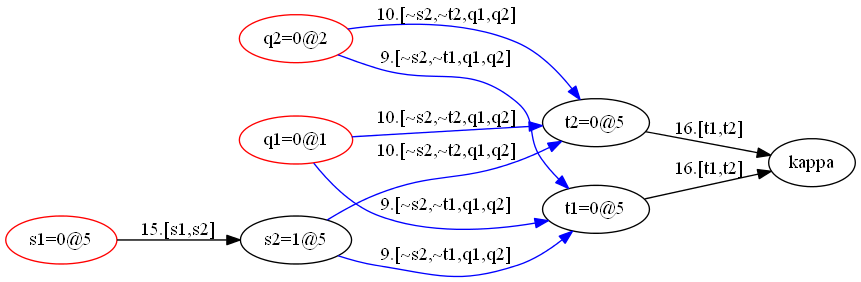
\includegraphics[keepaspectratio=true,width=\textwidth]{pebbles-color}
\end{center}
we see that the learned clause is:
\begin{verbatim}
Learned clause from resolution: [~s2,q1,q2]
\end{verbatim}

After learning the clause, three levels of decision assignments are
skipped:
\begin{verbatim}
Non-chronological backtracking to level: 2
Writing dot graph: 0
Skip decision assignment: s1=1@5
Skip decision assignment: r2=1@4
Skip decision assignment: r1=1@3
\end{verbatim}
(Clearly, the decision assignments for $r_1$ and $r_2$ are irrelevant to
the conflict.)

The subsequent decision assignments and unit propagation result in the
same conflict clause and a new learned clause with backtracking again to
level 2:

\begin{verbatim}
Conflict clause: [u1,u2]
Learned clause from resolution: [~t2,r1,r2]
Non-chronological backtracking to level: 2
\end{verbatim}

The same conflict appears again, but after learning the clause, the set
of clauses is immediately determined to be unsatisfiable because there
are no longer any decisions that have not been made:

\begin{verbatim}
Conflict clause: [u1,u2]
Learned clause from resolution: [~q1,p1,p2]
Unsatisfiable:
\end{verbatim}

The variable ordering is extremely important here. The default ordering
is lexicographic and we happened to put the first variables at the apex
of the graph. If we change the variable ordering to start with the
leaves and work up the graph, proving the formula unsatisfiable is much
less efficient even for mode NCB:

\begin{verbatim}
ncb:   units=26, decisions=21, conflicts=9
\end{verbatim}

%%%%%%%%%%%%%%%%%%%%%%%%%%%%%%%%%%%%%%%%%%%%%%%%%%%%%%%%%%%

\section{Seating guests at a table}

\begin{center}
These examples were contributed by Na'ama Tal and Nili Gilboa Luria.
\end{center}

\fl{tablea.pro, tableb.pro, tablec.pro}

Solving problems in the presence of constraints is an important
application of SAT solving because constraints are easily expressed as
logical formulas. The example we take is to compute a plan for seating
guests at a round table, where the constraints are of one of two forms:
Guest $g_i$ \emph{must} sit next to guest $g_j$ or guest $g_i$
\emph{refuses} to sit next to guest $g_j$. The examples will use a table
with six seats for six guests.

\subsection{Encoding the problem}

The atomic proposition \p{pij} is true iff guest $g_i$ sits in chair
$c_j$, $1 \leq i,j \leq 6$.

Each guest must sit in some chair, so we have six clauses of the form:
\begin{verbatim}
  [pi1, pi2, pi3, pi4, pi5, pi6]
\end{verbatim}
There is one clause for each $1 \leq i \leq 6$.

Similarly, no more than one guest can sit in any chair, so we have six
sets of clauses of the form:
\begin{verbatim}
  [~p1j, ~p2j], [~p1j, ~p3j], [~p1j, ~p4j], [~p1j, ~p5j], [~p1j, ~p6j], 
  [~p2j, ~p3j], [~p2j, ~p4j], [~p2j, ~p5j], [~p2j, ~p6j],  
  [~p3j, ~p4j], [~p3j, ~p5j], [~p3j, ~p6j], 
  [~p4j, ~p5j], [~p4j, ~p6j], 
  [~p5j, ~p6j]
\end{verbatim}
There is one set of clauses for each $1 \leq j \leq 6$.
 
To encode that $g_i$ refuses sit next to guest $g_j$, use a clause for
each of the two adjacent chairs $c_{k-1}$, $c_{k+1}$ (where addition are
subtraction are modulo 6):

\begin{displaymath}
p_{ik} \rightarrow \ngg p_{j(k-1)} \wedge \ngg p_{j(k+1)} \equiv
(\ngg p_{ik} \vee \ngg p_{j(k-1)} ) \wedge
(\ngg p_{ik} \vee \ngg p_{j(k+1)} ) 
\end{displaymath}
For example, if $g_1$  refuses to sit next to $g_2$, then if $g_1$ sits
in $c_1$, $g_2$ can't sit in $c_2$ or $c_6$:

\begin{verbatim}
  [~p11, ~p22], [~p11, ~p26]
\end{verbatim}
Each constraint gives rise to six pairs of clauses, one for each chair.

There are two ways to encode the constraint that guest $g_i$ must sit
next to guest $g_j$. One way is to take implications of the form:
\begin{displaymath}
p_{ik_{1}} \rightarrow \ngg p_{jk_{2}} \equiv
\ngg p_{ik_{1}} \vee \ngg p_{jk_{2}}
\end{displaymath}
for every pair of chairs $k_1, k_2$ that are \emph{not} adjacent. For
example, if $g_3$ must sit next to $g_4$, then if $g_3$ sits in $c_1$,
$g_4$ must sit in $c_6$ or $c_2$, \emph{not} in $c_3$, $c_4$ or $c_5$:

\begin{verbatim}
  [~p31, ~p43], [~p31, ~p44], [~p31, ~p45] 
\end{verbatim}
There will be six sets of three clauses, one set for each chair.

The second way is to directly encode the adjacency requirements; if
$g_i$ sits in $c_{k}$ then $g_j$ must sit in $c_{k-1}$ or $c_{k+1}$:
\begin{displaymath}
p_{ik} \rightarrow p_{j(k-1)} \vee p_{j(k+1)} \equiv
\ngg p_{ik} \vee p_{j(k-1)} \vee p_{j(k+1)}.
\end{displaymath}
In the example, if $g_3$ must sit next to $g_4$, then if $g_3$ sits in
$c_1$, $g_4$ must sit in $c_2$ or $c_6$:
\begin{verbatim}
  [~p31, p42, p46]
\end{verbatim}
There is one three-literal clause for each of the six chairs.


\subsection{Three problems}

The archive contains three problems for seating guests.

File \p{tablea.pro} encodes the constraints:
\begin{itemize}
\item $g_1$ refuses to sit next to $g_2$
\item $g_4$ refuses to sit next to $g_5$
\item $g_3$ must  sit next to $g_4$ 
\item $g_3$ must  sit next to $g_6$ 
\end{itemize}
and the first encoding of $g_i$ must sit next to guest $g_j$ is used.
The problem is satisfiable under the assignment:
\begin{verbatim}
  p16=1, p24=1, p32=1, p43=1, p55=1, p61=1
\end{verbatim}
and is solved in \emph{all} modes with the statistics:
\begin{verbatim}
  units=44, decisions=15, conflicts=2, learned clauses=0
\end{verbatim}

File \p{tableb.pro} encodes the constraints:
\begin{itemize}
\item $g_1$ refuses to sit next to $g_2$
\item $g_4$ refuses to sit next to $g_5$
\item $g_3$ must  sit next to $g_1$
\item $g_3$ must  sit next to $g_4$ 
\item $g_3$ must  sit next to $g_6$ 
\end{itemize}
and the second, more efficient, encoding of $g_i$ must sit next to guest
$g_j$ is used. The problem is unsatisfiable but there is still no
difference in the statistics in the different modes:
\begin{verbatim}
  units=759, decisions=120, conflicts=61, learned clauses=5
\end{verbatim}

File \p{tablec.pro} encodes the constraints:
\begin{itemize}
\item $g_1$ refuses to sit next to $g_2$
\item $g_3$ must  sit next to $g_4$
\item $g_4$ must  sit next to $g_5$
\item $g_5$ must  sit next to $g_6$ 
\end{itemize}
and the efficient encoding is used. This time, the three modes give
significantly different results:
\begin{verbatim}
  dpll: units=1187, decisions=286, conflicts=144
  cdcl: units=1016, decisions=232, conflicts=117, learned clauses=26
  ncb : units=926,  decisions=207, conflicts=92,  learned clauses=14
\end{verbatim}

The examples show that it is hard to predict when the advanced
algorithms improve performance.


%%%%%%%%%%%%%%%%%%%%%%%%%%%%%%%%%%%%%%%%%%%%%%%%%%%%%%%%%%%

\section{Graph coloring}\label{s.graph-color}

\fl{mcgregor.pro}

One of the most famous mathematical problems concerns the coloring of planar graphs, often called maps, such that no adjacent areas receive the same color.\footnote{This section is based on \cite[pp. 7, 134]{knuth-sat}} In 1976 was the Four Color Theorem proved that four colors are sufficient. Shortly before the proof appeared, Martin Gardner claimed \emph{five} colors were needed to color a map called the \emph{McGregor graph of order $10$}. This was one of a series of spoofs for April Fools day, though many reader were taken in.

The archive contains programs that use SAT solving to show that the McGregor graph of order $3$ (Figure~\ref{fig.mcgregor}) cannot be colored with three colors but can be colored with four colors.

The map has twelve areas. For each area, a clause is needed to ensure that the area is colored by at least one color, and a set of clauses is needed to require that adjacent areas are colored with different colors. Suppose that we are trying to find a four-coloring of the graph. The variables are \p{vnc}, where \p{n} is the label of an area and \p{c} is one of the colors. For area \p{22} in the graph, there is a clause:
\begin{verbatim}
  [v201,v202,v203,v204]
\end{verbatim}
requiring that at least one of the colors \p{1}, \p{2}, \p{3}, \p{4} be assigned to that area. The following clauses require that color \p{1} cannot be used \emph{both} for area \p{20} \emph{and} for one of \p{21}, \p{22}, \p{30}, \p{31}:
\begin{verbatim}
  [~v201,~v211], [~v201,~v221], [~v201,~v301], [~v201,~v311]
\end{verbatim}
the areas adjacent to area \p{20}. There are similar sets of clauses for colors \p{2}, \p{3} and \p{4}. Since we generated the clauses in ascending order of the labels of the areas, we do not have to include clauses like \verb+[~v201,~v111]+, because \verb+[~v111,~v211]+ was previously included and the clauses are commutative.

% The following diagram was generated using TikZ
% You can find the source in the file tikz.tex

\begin{figure}
\begin{center}
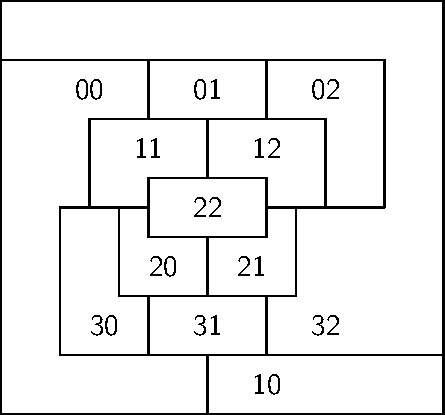
\includegraphics[width=.4\textwidth]{mcgregor3}
\caption{McGregor graph of order 3}\label{fig.mcgregor}
\end{center}
\end{figure}

Run the program and check that the variables assigned \p{1} define a correct four-coloring.

%%%%%%%%%%%%%%%%%%%%%%%%%%%%%%%%%%%%%%%%%%%%%%%%%%%%%%%%%%%

\section{Colored queens}\label{s.color-queens}

\fl{color-queens.pro}

Can you place $k$ colored queens on every square of an $n\times n$ board such that no color appears more than once in any row, column or diagonal? For a $4\times 4$ board, the left diagram below shows a failed attempt to assign four colors (A,B,C,D). Although no color appears more than once in any row or column, colors appear multiple times on the diagonals. In fact, there is no solution to the problem for four colors, but there are solutions for five colors (A,B,C,D,E) as seen in the right diagram:

\begin{center}
\unitlength=1.0pt
\begin{picture}(100,100)
  \put(0,0){\grid(80,80)(20,20)}
  \put( 0, 60){\makebox(20,20){A}}
  \put(20, 60){\makebox(20,20){D}}
  \put(40, 60){\makebox(20,20){C}}
  \put(60, 60){\makebox(20,20){B}}

  \put( 0, 40){\makebox(20,20){B}}
  \put(20, 40){\makebox(20,20){C}}
  \put(40, 40){\makebox(20,20){D}}
  \put(60, 40){\makebox(20,20){A}}

  \put( 0, 20){\makebox(20,20){C}}
  \put(20, 20){\makebox(20,20){B}}
  \put(40, 20){\makebox(20,20){A}}
  \put(60, 20){\makebox(20,20){D}}

  \put( 0, 0){\makebox(20,20){D}}
  \put(20, 0){\makebox(20,20){A}}
  \put(40, 0){\makebox(20,20){B}}
  \put(60, 0){\makebox(20,20){C}}
\end{picture}
\hspace{3em}
\begin{picture}(100,100)
  \put(0,0){\grid(80,80)(20,20)}
  \put( 0, 60){\makebox(20,20){E}}
  \put(20, 60){\makebox(20,20){D}}
  \put(40, 60){\makebox(20,20){C}}
  \put(60, 60){\makebox(20,20){B}}

  \put( 0, 40){\makebox(20,20){C}}
  \put(20, 40){\makebox(20,20){B}}
  \put(40, 40){\makebox(20,20){A}}
  \put(60, 40){\makebox(20,20){E}}

  \put( 0, 20){\makebox(20,20){A}}
  \put(20, 20){\makebox(20,20){E}}
  \put(40, 20){\makebox(20,20){D}}
  \put(60, 20){\makebox(20,20){C}}

  \put( 0, 0){\makebox(20,20){D}}
  \put(20, 0){\makebox(20,20){C}}
  \put(40, 0){\makebox(20,20){B}}
  \put(60, 0){\makebox(20,20){A}}
\end{picture}
\end{center}

Let the variables be \p{pijk} where \p{i}, \p{j} are the row and column of a square and \p{k} is the color assigned to that square. The following clauses require that each of the squares in the first row contain (at least) one of four colors:
\begin{verbatim}
  [p111, p112, p113, p114], 
  [p121, p122, p123, p124], 
  [p131, p132, p133, p134], 
  [p141, p142, p143, p144]
\end{verbatim}
Similar clauses are needed for the other rows.

For each square, we need \emph{exclusion clauses} which require that if a color appears in a square then it does not appear in any square in the same row, column and diagonal. Here are the exclusion clauses for \p{p111}, the literal that claims that the first square is colored \p{1}:
\begin{verbatim}
  [~p111, ~p121], [~p111, ~p131], [~p111, ~p141], 
  [~p111, ~p211], [~p111, ~p311], [~p111, ~p411],
  [~p111, ~p221], [~p111, ~p331], [~p111, ~p441]
\end{verbatim}
There are three more sets of these clauses for the other colors.

As you construct exclusion clauses for each successive square, their number decreases since the requirements are commutative. For example, once you have added \verb+[~p113,~p123]+ to require that squares \p{11} and \p{12} not both be colored with color \p{3}, you don't need \verb+[~p123,~p113]+.

Write sets of clauses to prove the obvious facts that you can't color a $2\times 2$ board with two or three colors, but you can with four colors.

%%%%%%%%%%%%%%%%%%%%%%%%%%%%%%%%%%%%%%%%%%%%%%%%%%%%%%%%%%%

\section{Tseitin graphs}\label{s.tseitin}

\fl{GenerateSatPRO.java, tseitin.pro}

G.S. Tseitin used formulas associated with graphs in his research on the
complexity of resolution.\footnote{See \cite[Section 4.5]{mlcs} for a
formal presentation of Tseitin formulas.} Consider the following
connected undirected graph whose vertices are labeled with 0 or 1 and
whose edges are labeled with letters:

\begin{center}
\unitlength=1.0pt
\begin{picture}(100,100)
\put(10,10){\framebox(80,80){\ }}
\put(10,10){\line(1,1){80}}
\put(0,0){\makebox(10,10){$0$}}
\put(45,0){\makebox(10,10)[b]{$t$}}
\put(90,0){\makebox(10,10){$0$}}
\put(0,45){\makebox(10,10)[l]{$q$}}
\put(40,45){\makebox(10,10)[l]{$r$}}
\put(90,45){\makebox(10,10)[r]{$s$}}
\put(0,90){\makebox(10,10){$0$}}
\put(45,90){\makebox(10,10)[t]{$p$}}
\put(90,90){\makebox(10,10){$1$}}
\end{picture}
\end{center}

The formula associated with this graph is defined as follows: for each vertex, construct the set of clauses whose atoms are the letters labeling the incident edges, such that the parity (sum modulo 2) of the number of negated literals is not equal to the label of the vertex:

\begin{verbatim}
[~p, q], [p, ~q],
[p, r, s], [~p, ~r, s], [~p, r, ~s], [p, ~r, ~s],
[~s, t], [s, ~t],
[~q, r, t], [q, ~r, t], [q, r, ~t], [~q, ~r, ~t]
\end{verbatim}

For example, since $\{p, r, s\}$ are incident with a vertex labeled 1, the number of negated literals in a cluase on these atoms has to be 0 or 2.

If the number of vertices labeled 1 is odd, the formula is unsatisfiable.

Let us look at the implication graph:

\begin{center}
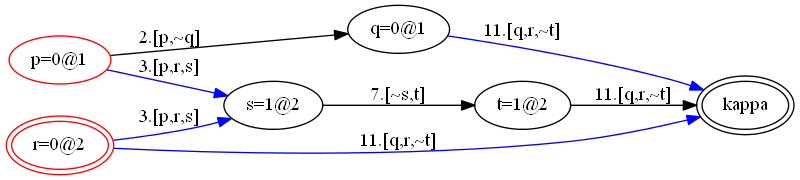
\includegraphics[keepaspectratio=true,width=\textwidth]{tseitin-ex-color}
\end{center}

The only dominator of the lowest decision node \verb+r=0@2+ is
the decision node itself. Since it is not implied by other decision
node, we cannot skip it in backtracking and the assignment \verb+r=1@2+
will have to be tried.

Another anomaly of this example is that the clause that would be learned
from the dominator is not the same as the one learned by resolution. The
former is \verb+[p,r]+, which is the complement of the dominator
decision node \verb+r=0@2+ and the decision node at a higher level
\verb+p=0@1+. The clause learned by resolution is obtained as follows:

\begin{verbatim}
Conflict clause: 11. [q,r,~t]
Resolvent: of [q,r,~t] and antecedent [~s,t] is [q,r,~s]
Resolvent: of [q,r,~s] and antecedent [p,r,s] is [q,p,r]
UIP: one literal r is assigned at level: 2
Learned clause from resolution: [q,p,r]
\end{verbatim}

This is a weaker clause than that defined by the dominator.

\bigskip

The archive includes programs for Tseitin clauses on the bipartite graphs $K_{2,2}, K_{3,3}, K_{4,4}$. These were generated by the Java program \texttt{GenerateSatPRO.java}.

%%%%%%%%%%%%%%%%%%%%%%%%%%%%%%%%%%%%%%%%%%%%%%%%%%%%%%%%%%%
%%%%%%%%%%%%%%%%%%%%%%%%%%%%%%%%%%%%%%%%%%%%%%%%%%%%%%%%%%%

\chapter{Bounded model checking}\label{ch.model}

\fl{bmc-generate-sem.pro, bmc-sem.pro}

Model checking a method for verifying the correctness of computer
hardware and software. A model checker inputs a formal description of a
system and a correctness claim and then searches for states in the
execution of the system that falsify the claim.

In \emph{explicit-state} model checkers, the reachable states of the
system are generated one-by-one and the correctness claim is evaluated
after each new state is evaluated. If the system has a finite number of
states, eventually the model checker will either find
a state falsifying the claim or declare that the claim is true in all
reachable states. Clever algorithms and optimized data structures ensure
that many real systems can be completely checked. For an overview of
explicit-state model checking (in particular, the \textsc{Spin} model
checker), see \cite{primer}.

\emph{Symbolic} model checkers represent the set of reachable states and
a correctness claim in a data structure and then perform computations on
this data structure, leading to a falsifying state or to a determination
that the correctness claim holds. In \emph{bounded model checking}, the
system and (the negation of) its correctness claim are represented by a
formula in propositional logic. If a SAT solver finds that the formula
is satisfiable, the exists a state that does not fulfill the correctness
claim. The formula has subformulas for each step in the computation.
Since a SAT solver expects to receive a finite formula, it is necessary
to limit \textit{a priori} the number of execution steps, hence
\emph{bounded} model checking. Fortunately, it is usually possibly to
determine a bound such that if the system is not correct, a state that
falsifies the correctness claim will be found within that bound. See
\cite{bmc} for a survey of bounded model checking.

\newpage

%%%%%%%%%%%%%%%%%%%%%%%%%%%%%%%%%%%%%%%%%%%%%%%%%%%%%%%%%%%

\section{Encoding a concurrent program as a SAT problem}

Consider the solution of the critical section problem using a semaphore:

\begin{center}
\begin{tabular}{|l|l|}
\hline
\multicolumn{2}{|c|}{s: semaphore := 1}\\\hline
process p & process q\\\hline
non-critical section & con-critical section \\
wait(s) & wait(s) \\
critical section & critical section \\
signal(s) & signal(s)\\\hline
\end{tabular}
\end{center}

There are four statements in each process, but the only statements that
affect the synchronization are the semaphore operations. The algorithm
can be represented as follows, where we agree that a process is in its
critical section if it is about to execute the signal operation:

\begin{center}
\begin{tabular}{|l|l|}
\hline
\multicolumn{2}{|c|}{s: semaphore := 1}\\\hline
process p & process q\\\hline
wait(s) & wait(s) \\
signal(s) & signal(s)\\\hline
\end{tabular}
\end{center}

Each state can be represented by an atom composed of three letters:
\p{w} or \p{s}---meaning \emph{at wait} or \emph{at signal}---for each
of the two processes, and \p{o} or \p{z}---meaning that the value of
\p{s} is one or zero. In addition, each atom will have a number: \p{0},
\p{1}, \p{2}, \p{3}, \ldots, for the steps of the execution. The initial
state is \p{wwo0}. The state \p{ssz5} means that after step 5 both
processes are at their signal instructions and the value of the
semaphore is zero. Of course, this means that mutual exclusion does
not hold so the program is not correct.

Notation: \verb=^= is conjunction, \verb=<->= is equivalence, \verb=+= is
exclusive or, \p{N} is a step, \p{N'} is the next step.

The initial state requires that the following formula be true:
\begin{verbatim}
(wwo0 ^ ~wwz0 ^ ~swo0 ^ ~swz0 ^ ~wso0 ^ ~wsz0 ^ ~sso0 ^ ~ssz0)
\end{verbatim}

The transitions of the system are represented by the following formula:
\begin{verbatim}
((wwoN <-> swzN') + (wwoN <-> wszN')) ^
(swoN <-> sszN') ^
(swzN <-> wwoN') ^
(wsoN <-> sszN') ^
(wszN <-> wwoN') ^
((sszN <-> wsoN') + (sszN <-> swoN'))
\end{verbatim}

The first formula says that in state \p{wwo}, \emph{either} process
\p{p} executes the wait instruction and reduces the value of \p{s} to 0
\emph{or} process \p{q} executes the wait instruction and reduces the
value of \p{s} to 0, \emph{but not both} (because we are using an
interleaving semantics of concurrency).\footnote{We assume a binary
semaphore with values 0 and 1 only, so signal cannot be executed if
the value of \p{s} is 1.}

Let us now guess that if there is a state that does not fulfill mutual
exclusion, it will occur within two steps. The formula representing
the computation consists of the conjunction of the formula for the
initial state and two copies of the formula for the transitions, one
with \p{N} equal to 0 and \p{N'} equal to 1 and another with \p{N} equal
to 1 and \p{N'} equal to 2.

Finally, take the conjunction of that formula together with the formula
representing the negation of the correctness claim: after 0, 1 or 2
steps, both processes are in their critical sections:\footnote{The value
of the semaphore is irrelevant.}

\begin{verbatim}
(ssz0 v sso0  v  ssz1 v sso1  v  ssz2 v sso2)
\end{verbatim}

The resulting formula is satisfiable if and only if mutual exclusion
does not hold within two steps.

The program \p{bmc-sem.pro} contains a predicate \p{generate} that takes
the above formula, converts it to CNF and writes (on file \p{bmc.pro})
the set of clauses in the correct form for running
\ls{}.\footnote{The program uses files \p{cnf.pro} and \p{ops.pro}
that were adapted from the program archive that accompanies
\cite{mlcs}.}

%%%%%%%%%%%%%%%%%%%%%%%%%%%%%%%%%%%%%%%%%%%%%%%%%%%%%%%%%%%

\section{Running the SAT solver on the encoding}

Load the file \p{bmc.pro}-sem in the \textsc{Prolog} compiler and run the predicate \p{bmc}. The result is that the formula is unsatisfiable, meaning that a violation of mutual exclusion does not happen within the first two steps. Of course, it is possible that it occurs after step 3, or step 4, or step 100, but from the structure of the program that seems unlikely.

The statistics for the three different modes are:
\begin{verbatim}
dpll: units=25, decisions=12, conflicts=7
cdcl: units=19, decisions=4,  conflicts=3, learned clauses=2
ncb:  units=16, decisions=3,  conflicts=2, learned clauses=2
\end{verbatim}
showing that the advanced algorithms are more efficient.

However, let us examine the trace in more detail. Since the original set
of clauses contains many unit clauses, the execution starts with a
series of unit propagations:
\begin{verbatim}
Propagate unit:  wwo0 (wwo0=1) derived from: [wwo0]
Propagate unit: ~wwz0 (wwz0=0) derived from: [~wwz0]
Propagate unit: ~swo0 (swo0=0) derived from: [~swo0]
Propagate unit: ~swz0 (swz0=0) derived from: [~swz0]
Propagate unit: ~wso0 (wso0=0) derived from: [~wso0]
Propagate unit: ~wsz0 (wsz0=0) derived from: [~wsz0]
Propagate unit: ~sso0 (sso0=0) derived from: [~sso0]
Propagate unit: ~ssz0 (ssz0=0) derived from: [~ssz0]
Propagate unit: ~ssz1 (ssz1=0) derived from: [swo0,~ssz1]
Propagate unit: ~wwo1 (wwo1=0) derived from: [swz0,~wwo1]
\end{verbatim}
Next, two decision assignments are made:
\begin{verbatim}
Decision assignment: sso1=0
Decision assignment: sso2=0
\end{verbatim}
but those seem strange. The initial state \p{wwo0} is one in which both
processes are at their wait operations at step 0, so why does the
algorithm start by assigning values to atoms associated with signal
operations at steps 1 and 2? By default, the algorithm makes decisions
assignment in lexicographic order of the atoms:\footnote{This list can
be displayed by selecting display option \p{variable}.}
\begin{verbatim}
Variables: [sso0,sso1,sso2,ssz0,ssz1,ssz2,swo0,swo1,swo2,swz0,swz1,swz2,
wso0,wso1,wso2,wsz0,wsz1,wsz2,wwo0,wwo1,wwo2,wwz0]
\end{verbatim}
By following our
intuition, let us change the order of the atoms by putting atoms in the
second line before those in the first line so that those beginning with
\p{w} are first:
\begin{verbatim}
set_order(
    [wso0,wso1,wso2,wsz0,wsz1,wsz2,wwo0,wwo1,wwo2,wwz0,
     sso0,sso1,sso2,ssz0,ssz1,ssz2,swo0,swo1,swo2,swz0,swz1,swz2]).
\end{verbatim}
Now, the algorithm in dpll mode is more efficient than it was in ncb mode!
\begin{verbatim}
dpll: units=14, decisions=2, conflicts=2
\end{verbatim}

This demonstrates that there is an element of nondeterminism in these
algorithms for SAT solving. Since it would not be tractable to try all
permutations of the order of the variables, there remains an element of
``luck'' when you choose an ordering arbitrarily, at random or using
 heuristics.




\bibliographystyle{plain}
\bibliography{learnsat}
\end{document}
